%\documentclass[12pt,a4paper,oneside]{report}             % Single-side
\documentclass[12pt,a4paper,twoside, openright]{report}  % Duplex

%\PassOptionsToPackage{chapternumber=Huordinal}{magyar.ldf} %betuvel a fejezetek szama
\usepackage{t1enc}
%\usepackage[latin2]{inputenc}
\usepackage{amsmath}
\usepackage{amssymb}
%\usepackage{amsfonts}
%\usepackage{enumerate}
%\usepackage[thmmarks]{ntheorem}
\usepackage{graphics}%s
\usepackage{epsfig}
\usepackage{color}

%\usepackage{fancyhdr}
%\usepackage{lastpage}
\usepackage{anysize}
\usepackage[magyar]{babel}
\usepackage[utf8]{inputenc}
\usepackage{sectsty}
\usepackage{setspace}  % Ettol a tablazatok, abrak, labjegyzetek maradnak 1-es sorkozzel!
\usepackage[hang]{caption}
\usepackage{hyperref}

%\usepackage{psfrag}
\usepackage{subfig}
\usepackage{float} % ezzel lehet helybe rakni az abrat

\usepackage{array}
%\usepackage{multirow}
\usepackage{enumerate}
\usepackage{listings}
\usepackage{gensymb}
%\usepackage{mdwlist}
%\makecompactlist{myitemize*}{itemize}

%\numberwithin{equation}{chapter}
\usepackage{todonotes}
\usepackage{changebar}

%--------------------------------------------------------------------------------------
% Main variables
%--------------------------------------------------------------------------------------
\newcommand{\vikszerzo}{Bakró Nagy István}
\newcommand{\vikkonzulens}{Reichardt András}
\newcommand{\vikcim}{AFM-es felületi töltéssűrűség mérésének szimulációja}
\newcommand{\viktanszek}{Szélessávú Hírközlés és Villamosságtan Tanszék}
\newcommand{\vikdoktipus}{TDK dolgozat}
\newcommand{\vikdepartmentr}{Szélessávú Hírközlés és Villamosságtan Tanszék}

%--------------------------------------------------------------------------------------
% Page layout setup
%--------------------------------------------------------------------------------------
% we need to redefine the pagestyle plain
% another possibility is to use the body of this command without \fancypagestyle
% and use \pagestyle{fancy} but in that case the special pages
% (like the ToC, the References, and the Chapter pages)remain in plane style

\pagestyle{plain}
%\setlength{\parindent}{0pt} % áttekinthet?bb, angol nyelv? dokumentumokban
% jellemz? \setlength{\parskip}{8pt plus 3pt minus 3pt} % áttekinthet?bb, angol nyelv? dokumentumokban jellemz?
\setlength{\parindent}{30pt} % magyar nyelv? dokumentumokban jellemz?
\setlength{\parskip}{0pt}    % magyar nyelv? dokumentumokban jellemz?

\marginsize{35mm}{25mm}{15mm}{15mm} % anysize package
\setcounter{secnumdepth}{0}
\sectionfont{\large\upshape\bfseries}
\setcounter{secnumdepth}{2}
\singlespacing
\frenchspacing

%--------------------------------------------------------------------------------------
%	Setup hyperref package
%--------------------------------------------------------------------------------------
\hypersetup{
    %bookmarks=true,            % show bookmarks bar?
    %unicode=false,             % non-Latin characters in Acrobat’s bookmarks
    %pdftitle={\vikcim},        % title
    %pdfauthor={\vikszerzo},    % author
    %pdfsubject={\vikdoktipus}, % subject of the document
    %pdfcreator={\vikszerzo},   % creator of the document
    pdfproducer={Producer},    % producer of the document
    pdfkeywords={keywords},    % list of keywords
    pdfnewwindow=true,         % links in new window
    %pdfborder={1 2 3},
    colorlinks=true,           % false: boxed links; true: colored links
    linkcolor=black,           % color of internal links
    citecolor=black,           % color of links to bibliography
    filecolor=black,           % color of file links
    urlcolor=black,             % color of external links
    breaklinks=true
}

%--------------------------------------------------------------------------------------
% Set up listings
%--------------------------------------------------------------------------------------
\lstset{
	basicstyle=\scriptsize\ttfamily, % print whole listing small
	keywordstyle=\color{black}\bfseries\underbar, % underlined bold black keywords
	identifierstyle=, 					% nothing happens
	commentstyle=\color{white}, % white comments
	stringstyle=\scriptsize\sffamily, 			% typewriter type for strings
	showstringspaces=false,     % no special string spaces
	aboveskip=3pt,
	belowskip=3pt,
	columns=fixed,
	backgroundcolor=\color{lightgray},
} 		
\def\lstlistingname{lista}	

%--------------------------------------------------------------------------------------
%	Some new commands and declarations
%--------------------------------------------------------------------------------------
\newcommand{\code}[1]{{\upshape\ttfamily\scriptsize\indent #1}}

% define references
\newcommand{\ud}{\ \mathrm{d}}
\newcommand{\mhat}[1]{\mathrm{\hat{#1}}}
\renewcommand{\vec}[1]{\overrightarrow{\mathrm{#1}}}

\DeclareMathOperator*{\argmax}{arg\,max}
%\DeclareMathOperator*[1]{\floor}{arg\,max}
\DeclareMathOperator{\sign}{sgn}
\DeclareMathOperator{\rot}{rot}
\definecolor{lightgray}{rgb}{0.95,0.95,0.95}

\author{\vikszerzo}
\title{\viktitle}
%--------------------------------------------------------------------------------------
%	Setup captions
%--------------------------------------------------------------------------------------
%\captionsetup[figure]{
%labelsep=none,
%font={footnotesize,it},
%justification=justified,
%width=.75\textwidth,
%aboveskip=10pt}

\renewcommand{\captionlabelfont}{\small\bf}
\renewcommand{\captionfont}{\footnotesize\it}

%--------------------------------------------------------------------------------------
% Table of contents and the main text
%--------------------------------------------------------------------------------------
\begin{document} 
\singlespacing
%\include{guideline}


%\pagenumbering{arabic}
%\pagenumbering{roman}
\onehalfspacing
\setcounter{page}{999}
%--------------------------------------------------------------------------------------
%	The title page
%--------------------------------------------------------------------------------------
\begin{titlepage}
\begin{center}

\includegraphics[height=42mm,keepaspectratio]{figures/eps/BMElogo.eps}\\
\vspace{0.3cm}
\textbf{Budapesti Műszaki és Gazdaságtudományi Egyetem}\\
\textmd{Villamosmérnöki és Informatikai Kar}\\
\textmd{\viktanszek}\\[5cm]

\vspace{0.4cm}
{\huge \bfseries \vikcim}\\[0.8cm]
\vspace{0.5cm}
\textsc{\Large \vikdoktipus}\\[4cm]

\begin{tabular}{cc}
 \makebox[7cm]{\emph{Készítette}} & \makebox[7cm]{\emph{Konzulens}} \\
 \makebox[7cm]{\vikszerzo} & \makebox[7cm]{\vikkonzulens}
\end{tabular}

\vfill
{\large \today}
\end{center}
\end{titlepage}
\clearpage
\null\newpage

\pagenumbering{roman}
\setcounter{page}{1}
\pdfbookmark{\contentsname}{toc}
\tableofcontents%\addcontentsline{toc}{chapter}{Tartalomjegyzék}
%\include{declaration}

%--------------------------------------------------------------------------------------
% Feladatkiiras (a tanszeken atveheto, kinyomtatott valtozat)
%--------------------------------------------------------------------------------------
\clearpage
\begin{center}
\large
\textbf{Kivonat}
\end{center}
\addcontentsline{toc}{chapter}{Kivonat}

Atomerő mikroszkóppal való fémezett felületű minta felületi töltéssûrûségének mérése során kritikus a tû és a minta közötti kapacitás ismerete.
A kapacitás értékét közelítések mellett lehetséges analitikusan kifejezni.
Numerikus szimulációval pontosabban ismerhetjük az értékét, ezáltal a felbontás nõ és a mérési zaj csökken.

A szimuláció során a lehetséges párhuzamosításokat felhasználva a számítási idõt elfogadhatóra csökkentettük,
ami akár online feldolgozást is lehetõvé teszi.

Atomerő mikroszkóppal való fémezett felületű minta felületi töltéssűrűségének
mérése során kritikus a tű és a minta közötti kapacitás ismerete.
A kapacitás értékét közelítések mellett lehetséges analtikusan kifejezni.
Numerikus szimulációval pontosabban ismerhetjük az értékét, ezáltal nagyobb
felbontás is érhető el.
A szimuláció során a lehetséges párhuzamosításokat felhasználva a számítási időt
elfogadhatóra csökkentettük.


\clearpage
\begin{center}
\large
\textbf{Abstract}
\end{center}
\addcontentsline{toc}{chapter}{Abstract}

The measurement of the surface charge density can be achived by Atomic Force Microscope (AFM).
The common method is the two-pass technic, which main goal is to seperate the net force acting upon the tip into components.
To do so we have to express the tip-sample capacitance, which is critical respectivly to the measurements accuracy.

The value of the capacitance can be expressed analitically, but with some strong neglecting.

We are presenting the accelerated simulation of this capacitance using GPU's programmed in
OpenCL's parallel framework.

 \clearpage

\pagenumbering{arabic}
\setcounter{page}{1}

%----------------------------------------------------------------------------
\chapter{Bevezetés}
%----------------------------------------------------------------------------
	1986-ban Binning demonstrálta az atomerő mikroszkóp (AFM) ötletét \cite{Binnig1986}, ami mára 
	a nanotechnológia egyik legfontosabb eszköze képalkotásra használható képalkotásra, nanolitográfiára és 
	adott anyag alakítására \cite{Vasic2013}.
	Az AFM apparátusa az adott minta felületé és pásztázó kantilever végére erősített tű 
	kölcsönhatásának vizsgálatát végzi. (lásd \ref{fig:tip-sample}. ábra)
	A felület és a tű közötti domináns kölcsönhatás határozza meg, hogy az anyag melyik fizikai
	mennyiségét kaphatjuk meg.
	\begin{figure}[H]
		\centering
		\subfloat[Az AFM apparátusa]{
			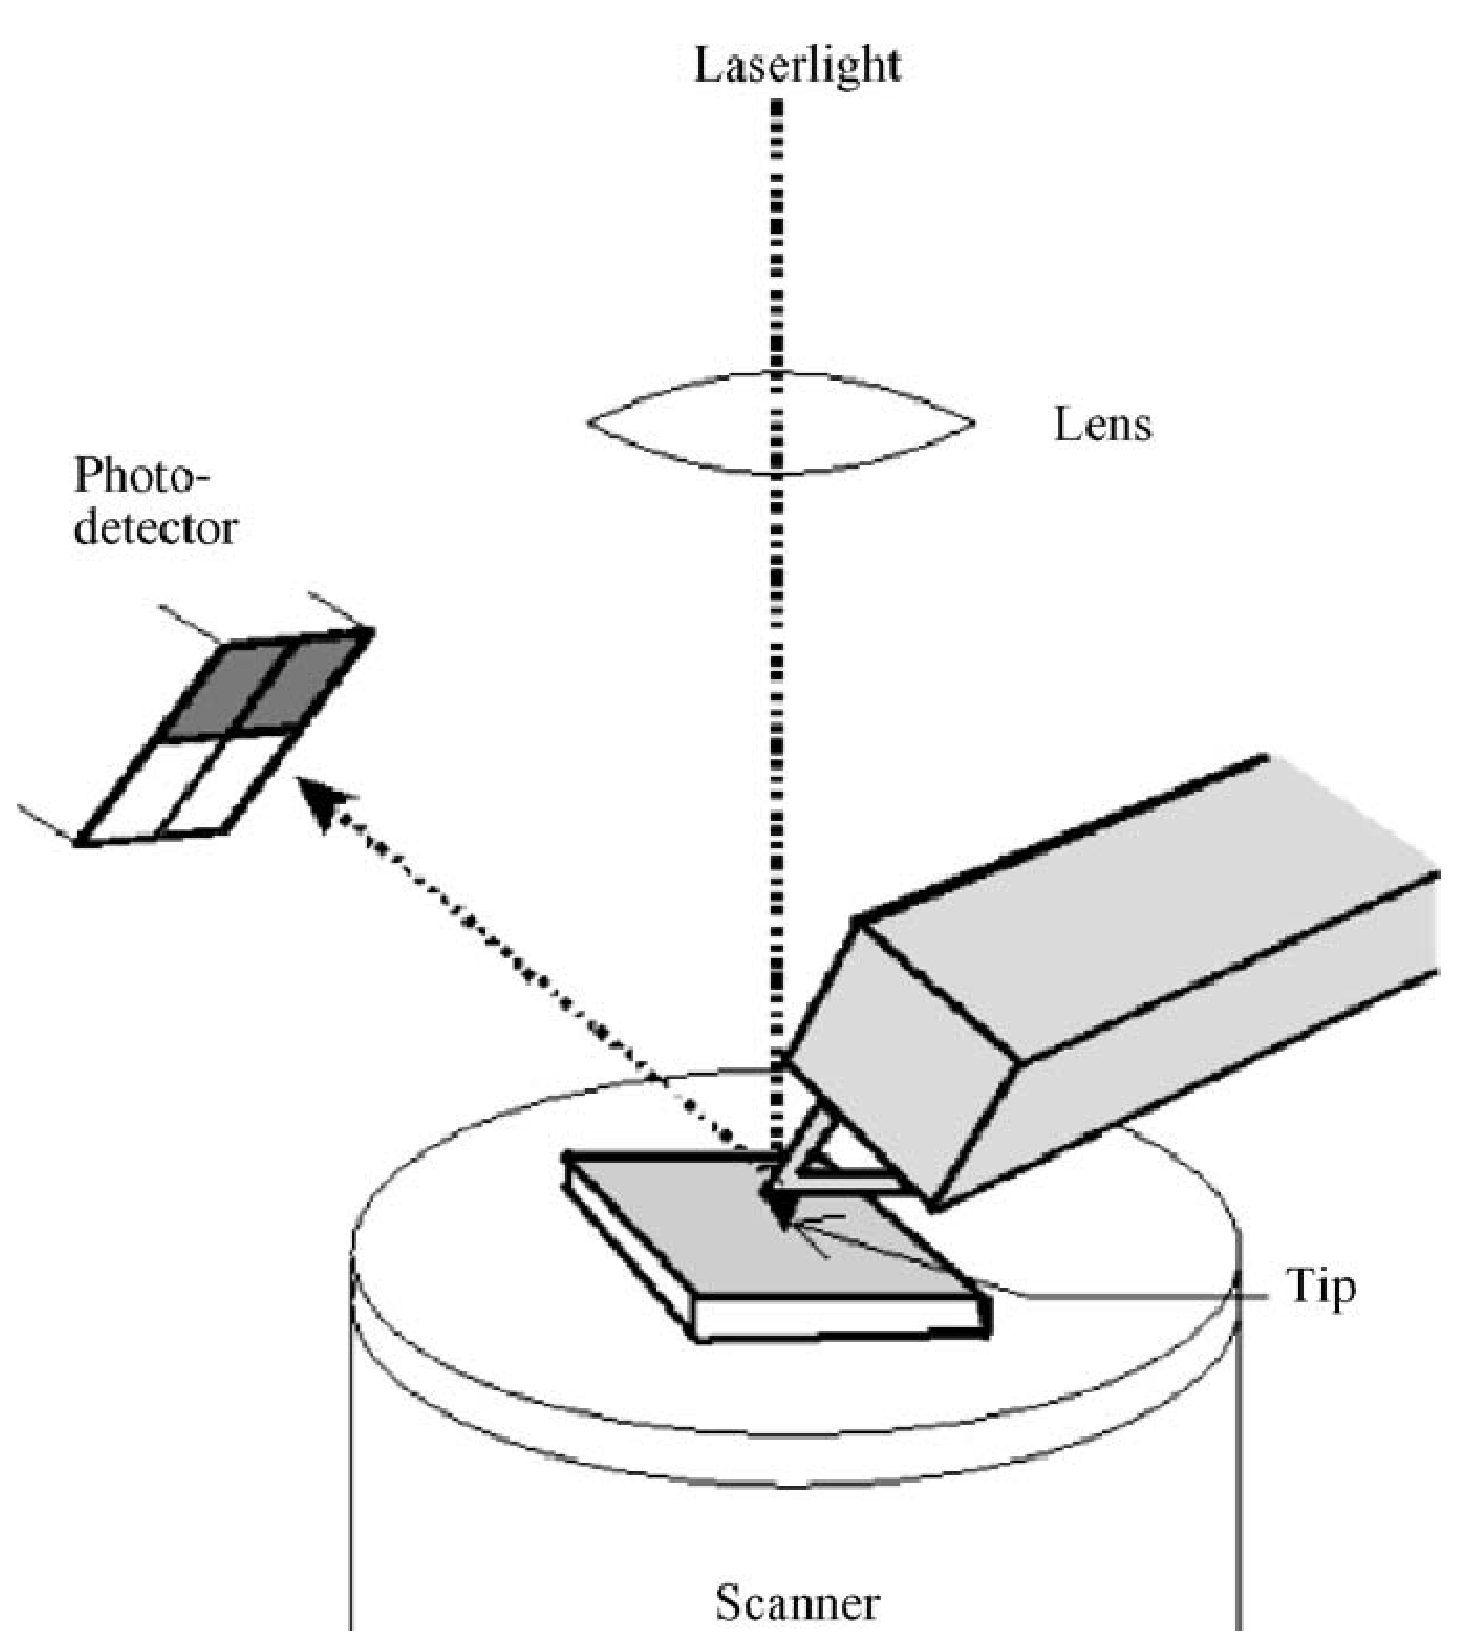
\includegraphics[width=0.4\columnwidth]{figures/eps/AFM.eps}%
			\label{fig:afm}
		}
		\hfil
		\subfloat[A tű és minta modellje]{
			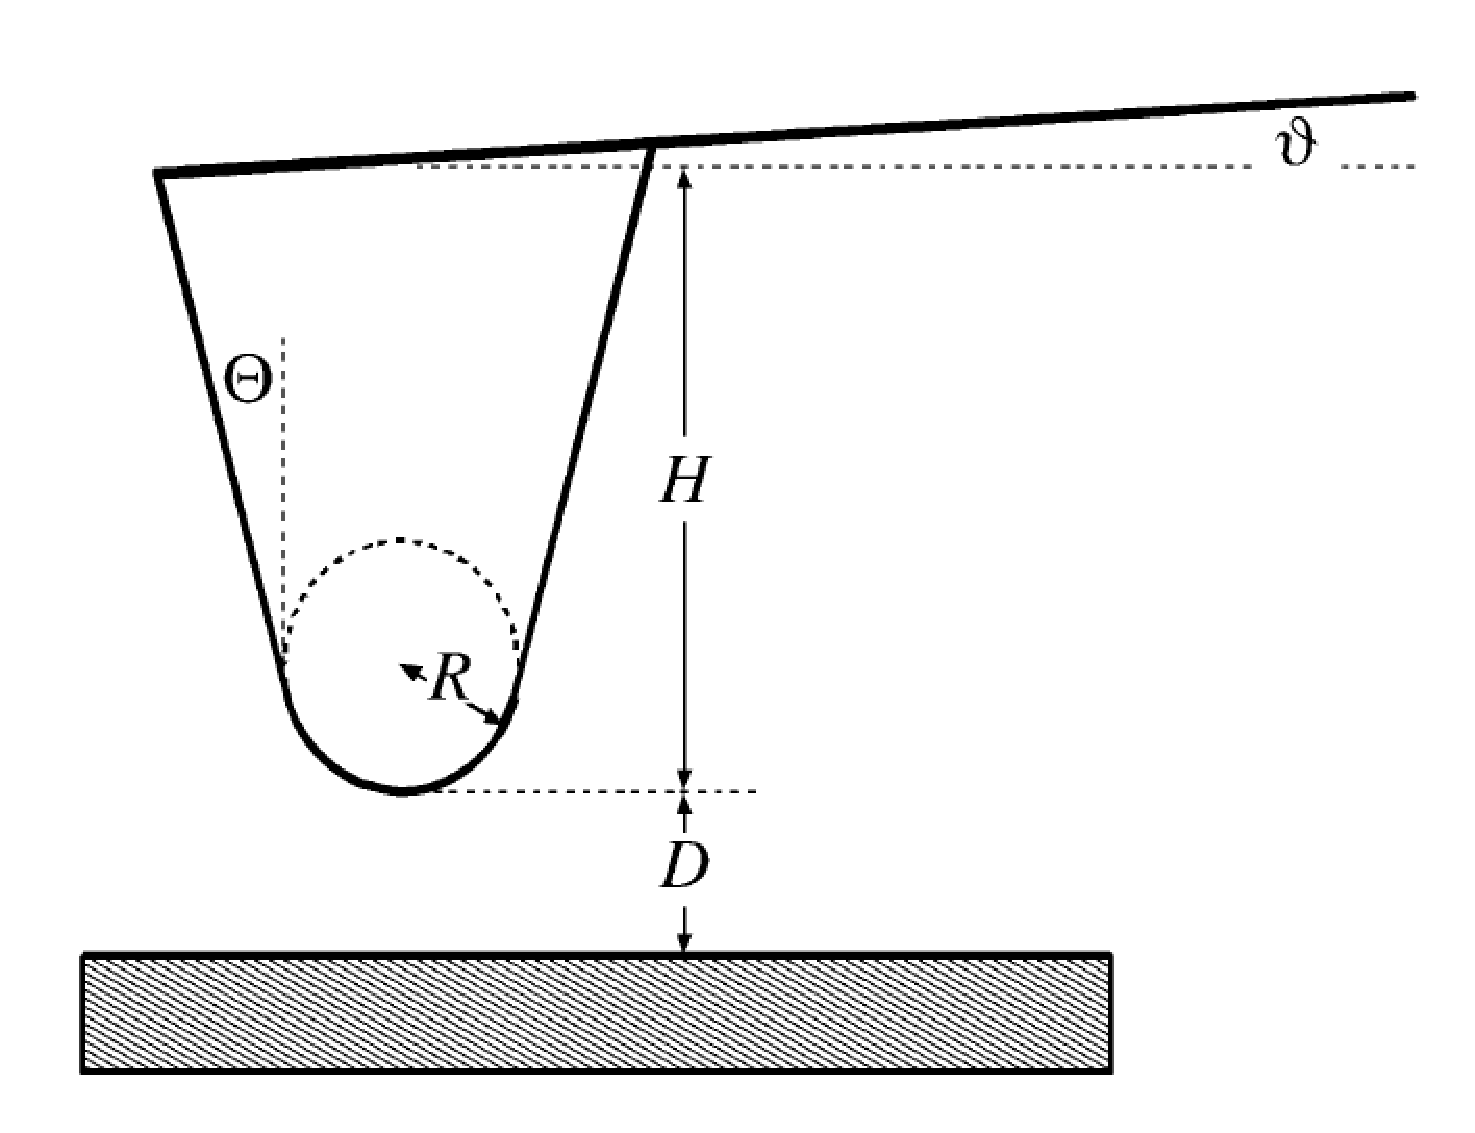
\includegraphics[width=0.4\columnwidth]{figures/eps/tip-sample.eps}
			\label{fig:tip-sample}
		}
		\caption{Az AFM apparátusa látható az (a) ábrán. A lázernyaláb
		a tű felületéről tükröződve egy fotódetektorra irányul. A tű pozícióját ez alapján nagy pontossággal ismerjük. A
		(b) ábrán a minta és a felette lévő tű modellje látható a kapacitás analitikus számításához.
		A tű $R$ sugarú $H$ magasságú és $D$ távolságra van a mintától. (Forrás: \cite{Butt20051})}
		\label{fig:fig_sim}
	\end{figure}
	Az AFM felhasználása kontakt illetve kopogtató üzemmódú lehet. A kontakt mód során a
	felületen végighúzzuk a tűt és mérjük a $z$ irányú elmozdulását. Így képesek vagyunk a minta
	felületén lévő atomok elrendezéséről magasságtérképet adni.
	Kopogtató mód \cite{Martin1987} során a tűt elemeljük a mintától és $f$ frekvenciával rezegtetjük.
	A letapogatás során az  átlagos minta-tű távolságot a kontakt módú magasságtérkép felhasználásával
	konstans értéken tartjuk.
	A kantilever dinamikáját ismerve a rezegtetés frekvenciájának eltéréséből
	számítható a tűre ható erő. Ezen erő nagyságát befolyásoló tényezők:
	\begin{enumerate}[a)]
		\item a minta és a tű kapacitására kapcsolt feszültség,\label{cap_force}
		\item a minta felületi töltéssűrűség eloszlása,\label{sc_force}
		\item Van der Waals erő.\label{vdw_force}
	\end{enumerate}
	A dolgozatban a felületi töltéssűrűség mérését tekintem célnak.
	
	A \cite{Butt1991Dec, Butt20051} szerint az erő \ref{cap_force} komponensét a minta és a tű közötti
	kapacitásból az \eqref{eq:capforce} szerint származtathatjuk.
	\begin{equation}\label{eq:capforce} 
	F_{s} = -\frac{\ud E}{\ud D} = -\frac{\ud (CV^2 /2)}{\ud D} = -\frac12 \frac{\ud C}{\ud D} V^2   
	\end{equation}
	Ha a minta pásztázása során ezen \ref{cap_force} erőkomponens konstansnak mondható, tehát a felületi
	érdesség és a távolság pontatlansága elhanyagolhatóan kicsi, akkor a töltéssűrűség mérésében ez állandó hibát okoz. ami
	eliminálható.
	Az \eqref{eq:capforce} számításában a kritikus elem a kapacitás értéke, amit numerikus számítás
	mellőzése esetén a \cite{Hudlet1998} szerinti analitikus eredményt használhatjuk fel.
	A tű formáját a \ref{fig:tip-sample} ábra szerintinek veszi és a mintát sík felületnek feltételezi.
	A tűre vonatkozó feltételezés legtöbb esetben helyénvaló, viszont a minta nagyfokú érdessége és változatossága végett érvényét
	veszti. Szemléltetését a \ref{fig:terkep_anim} ábrán lehet látni. 
	Ilyen esetben a kapacitás értéke mintáról mintára változik és állandó hiba helyett, a mérést zajként terheli.
	\begin{center}
		Ezen zaj kiküszöbölése a kapacitás numerikus szimulációjával lehetséges.
	\end{center}
	A probléma ezzel, hogy ezen szimulációt minden egyes mérési pontban el kell végezni, aminek a kivitelezése
	csak multiprocesszoros környezetben lehetséges elfogadható idő alatt.
	
	\begin{figure}[!hp]
		\begin{center}
		\subfloat[1. pillanat]{
			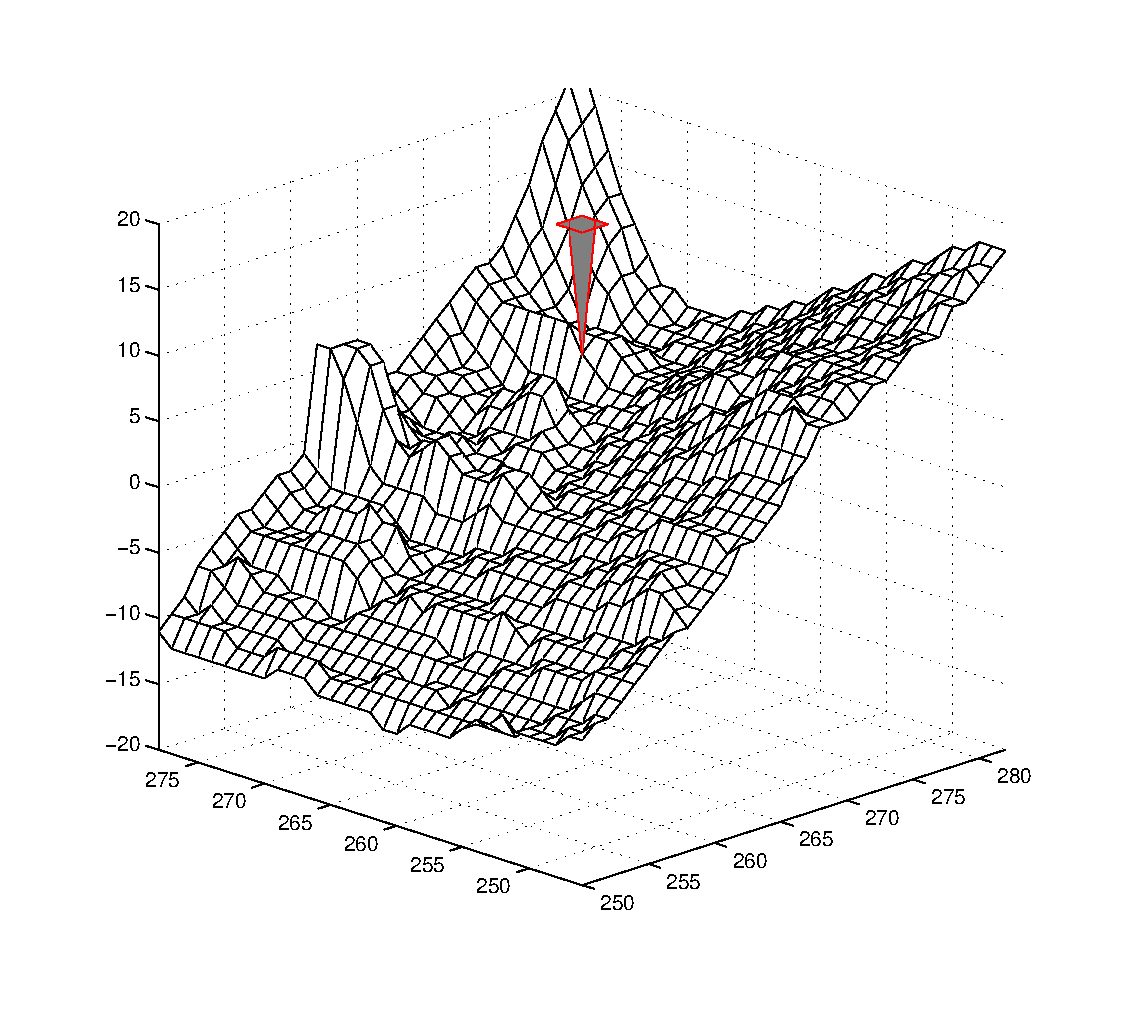
\includegraphics[height=0.22\paperheight]{figures/eps/el_1.eps}%
			%\label{fig:afm}
		}\\
		\subfloat[2. pillanat]{
			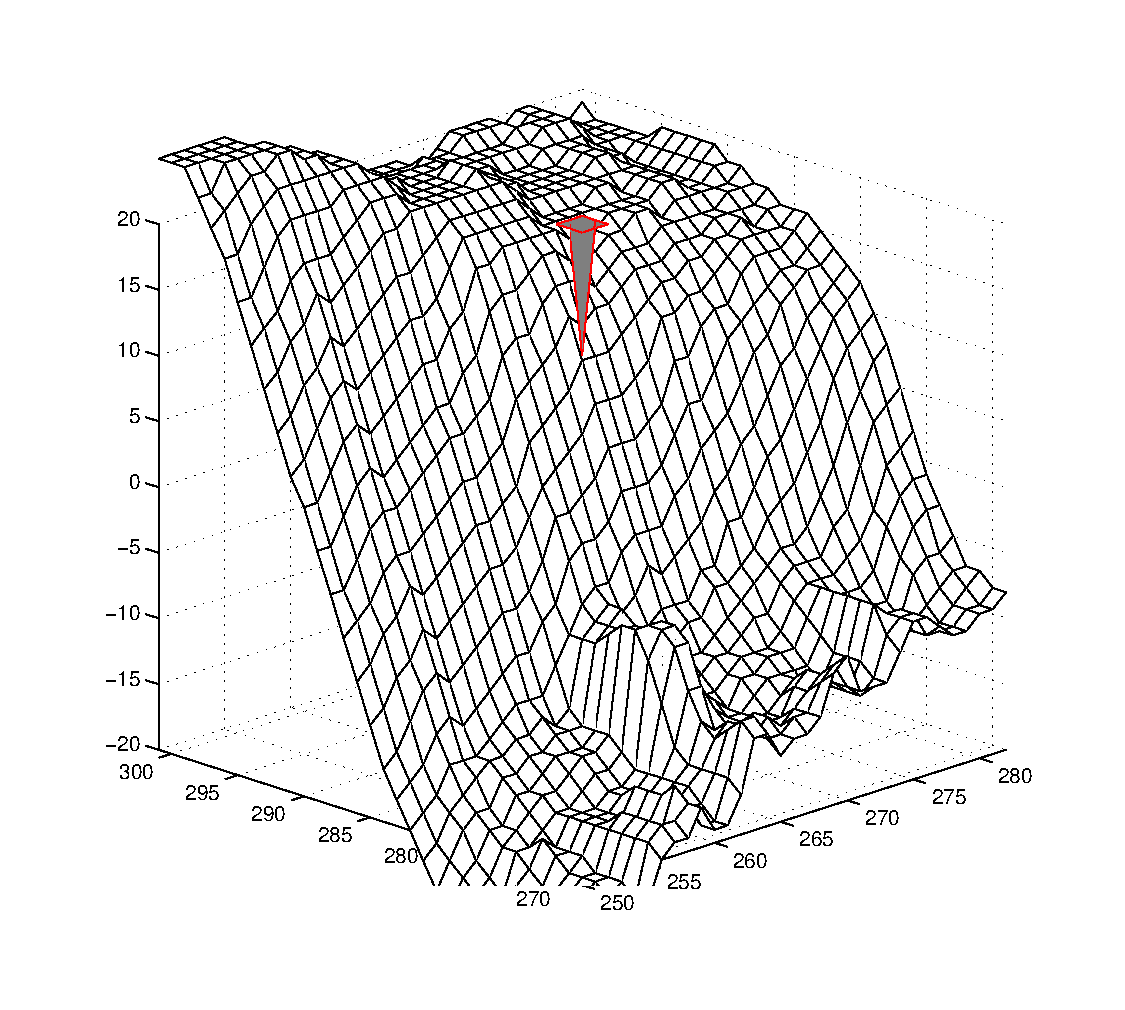
\includegraphics[height=0.22\paperheight]{figures/eps/el_2.eps}%
			%\label{fig:afm}
		}\\
		\subfloat[3. pillanat]{
			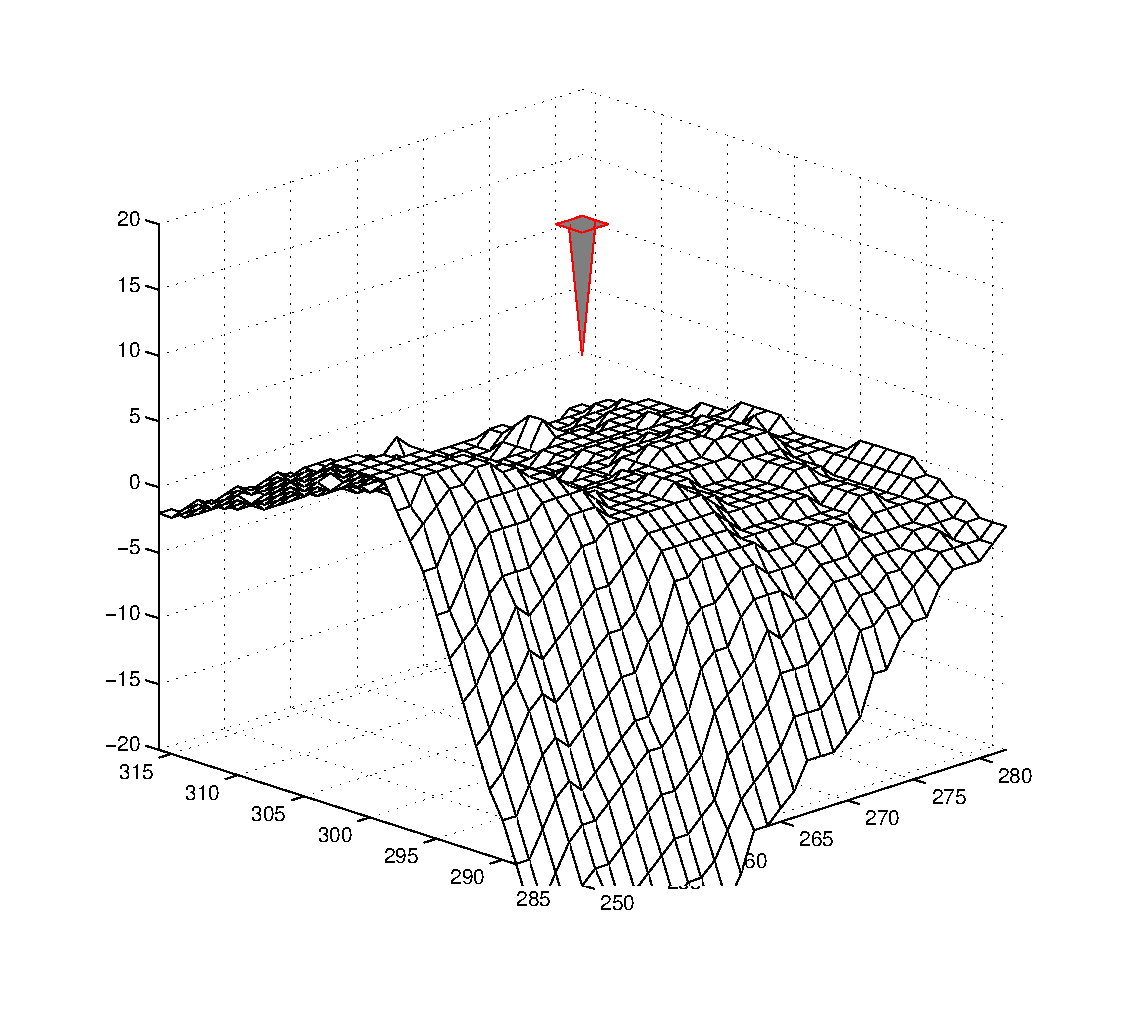
\includegraphics[height=0.22\paperheight]{figures/eps/el_3.eps}%
			%\label{fig:afm}
		}\\
		\caption{A magasságtérkép változása a második mérés során fix pozíciójú tű esetén.}
		\label{fig:terkep_anim}
		\end{center}
	\end{figure}
%----------------------------------------------------------------------------
\chapter{A feladat} \label{sec:feladat}
%----------------------------------------------------------------------------
	A minta egy fémezett felület, aminek magasságtérképét mérések eredményeként 
	adott pontossággal ismerjük.
	A magasságmérések egy négyzetes háló felett történtek, amelynek mindkét irányában
	$\delta_x = \delta_y \simeq 120 nm$ azonos a felbontása
	A magasságmérés függőleges pontossága $\delta_z \simeq 20nm$ volt.
	A töltéssűrűség méréséhez szükséges második pásztázás során a tűt a mintához képest $V_{tu} = 500 mV$ potenciálra kapcsoljuk.
	Illetve a fémezett felülettől közel azonos távolságra rezegtetjük és a (hosszú hegyes) tűre ható erőt mérjük.
	
	\noindent A dolgozatban felhasznált magasságtérkép-mérési eredmény (\ref{fig:felulet}. ábra) egy
	$512\times512$ méretű szürkeárnyalatos *.tiff állomány, amely értéke $0-255$-ig terjed.
	A mérőberendezés adatlapja alapján és a mérés végén megjelenített konstansokkal lehetséges a kép skálázása.
	
	\begin{figure}[!h]
		\centering
		\subfloat[Mérési eredmény]{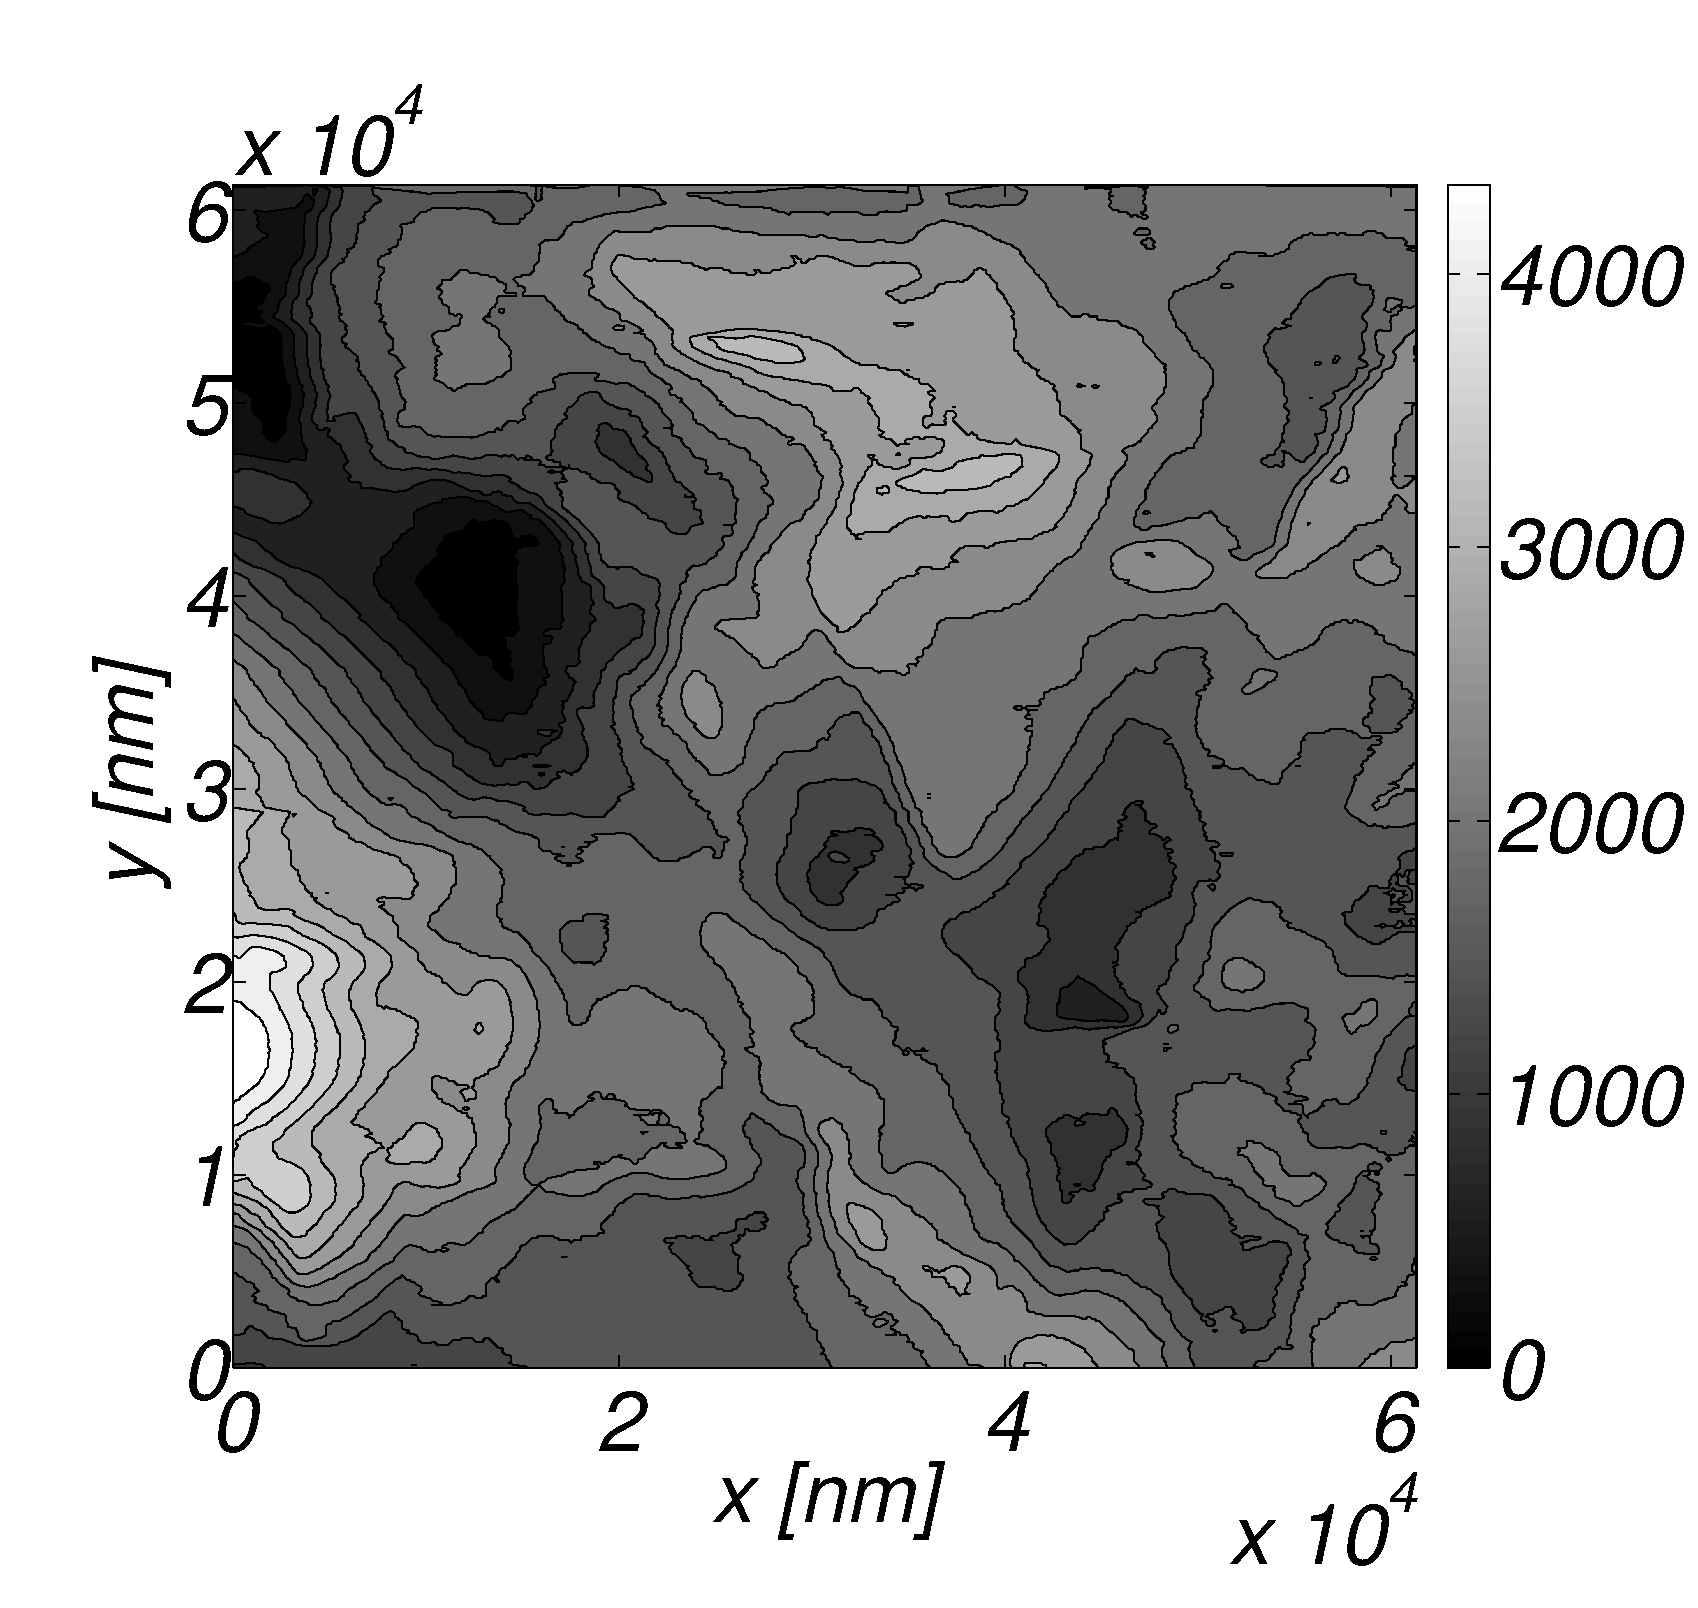
\includegraphics[width=0.6\columnwidth]{figures/eps/newafm_total.eps}%
		\label{fig:afm_total}}
		\hfil
		\subfloat[Mérés részlete]{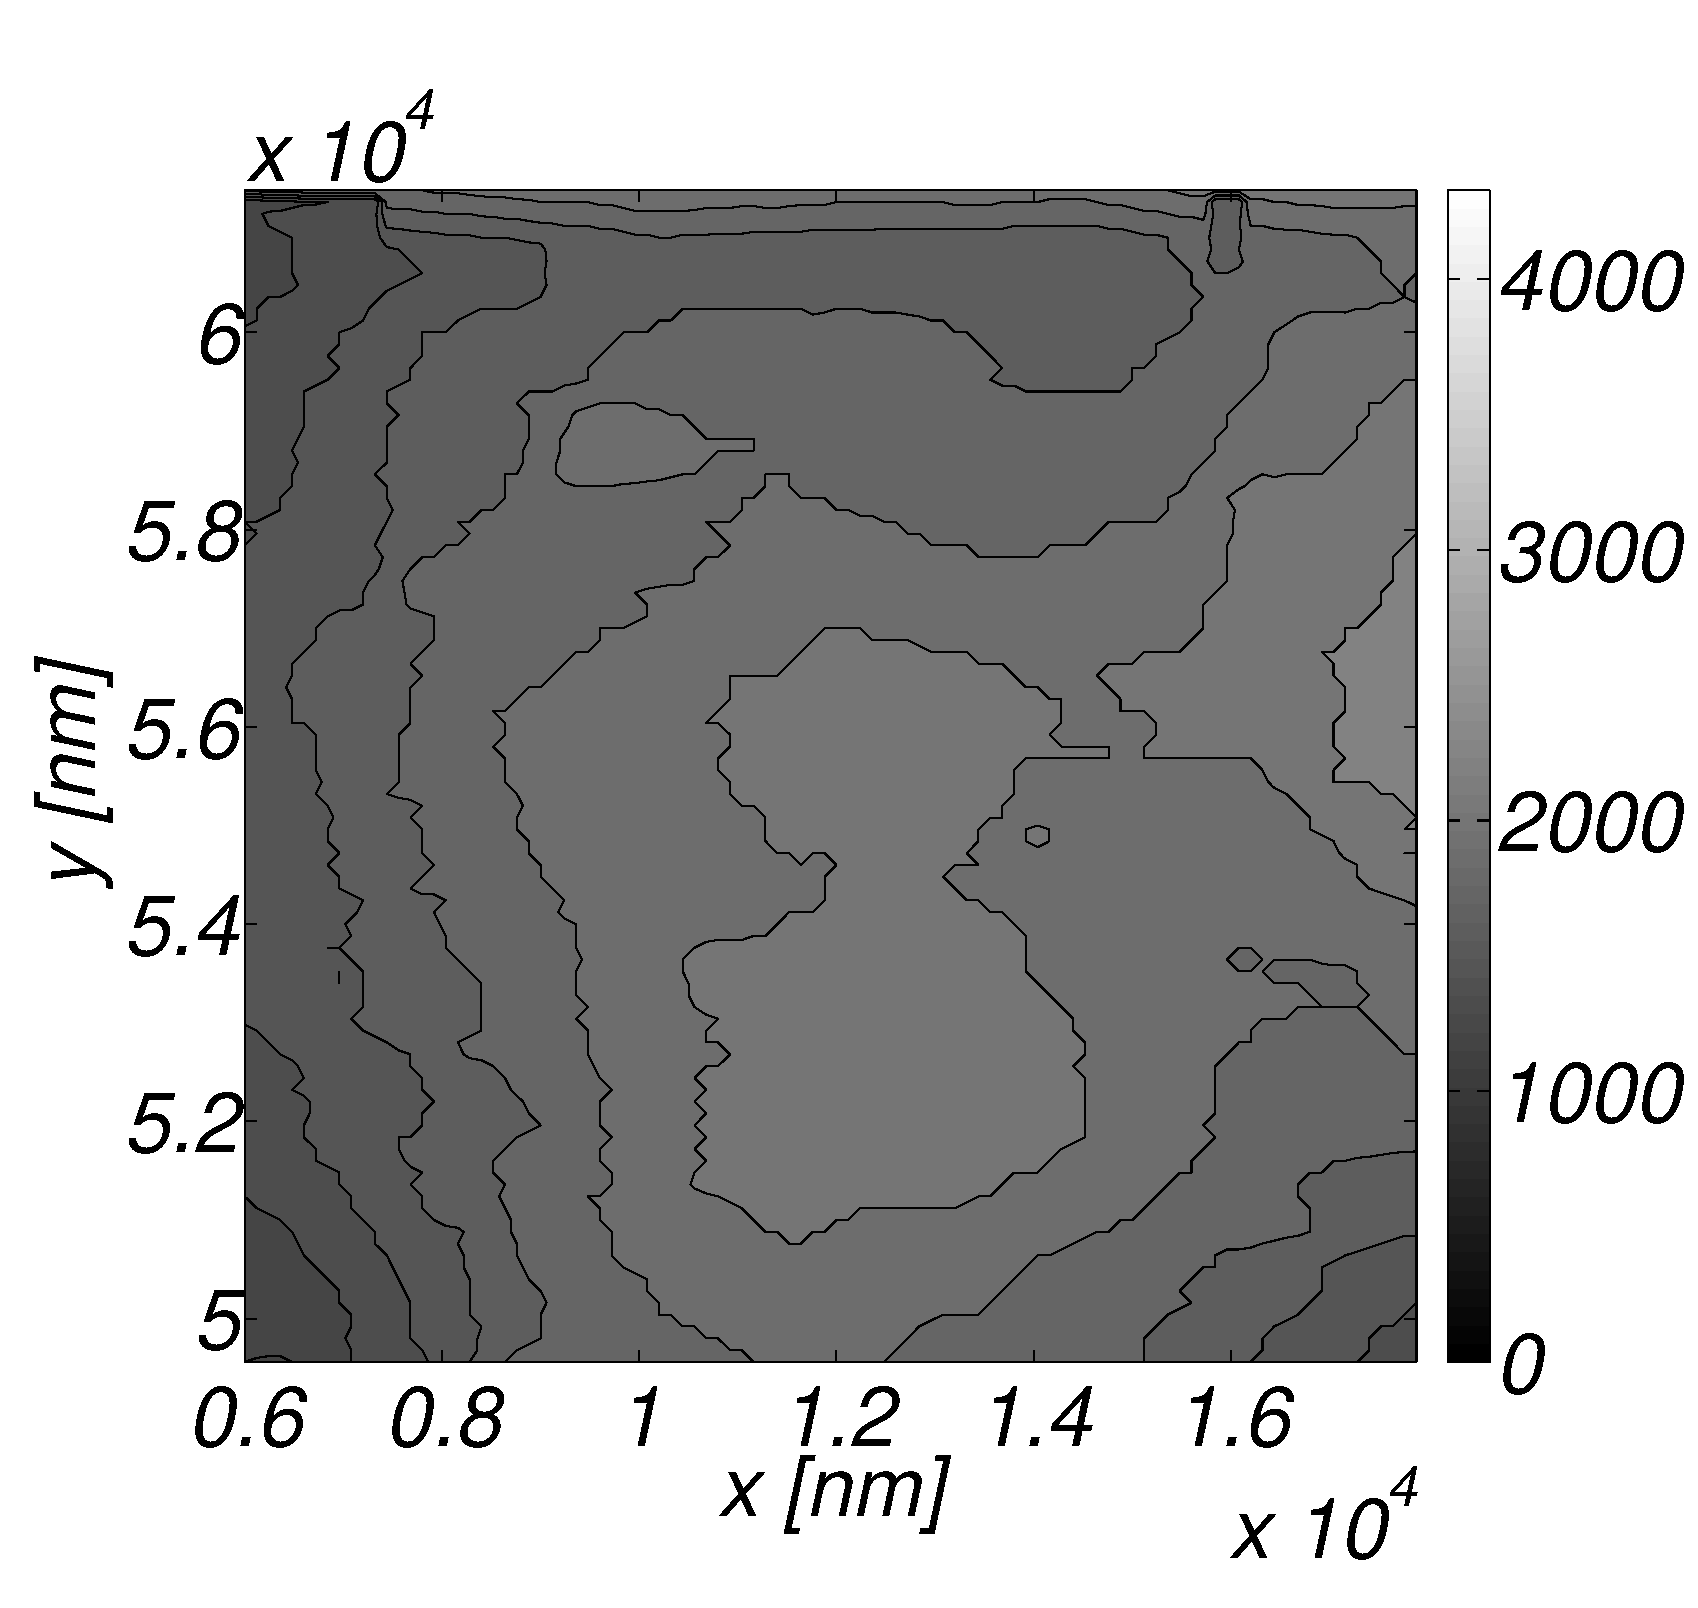
\includegraphics[width=0.3\columnwidth]{figures/eps/newafm200.eps}%
		\label{fig:afm200}}
		\caption{Méréssel kapott magasságtérkép. Felbontás $d_x=d_y=120nm \ d_z=18.03nm$}
		\label{fig:felulet}
	\end{figure}
	
	\noindent
	A dolgozat céljául egy olyan szimulátor építését tűztem ki, amely segítségével közel valós időben 
	lehetséges a mérés alapján a felületi töltéseloszlásról a mérőeszköz pontosságánál finomabb felbontást elérni.
	
	
	
\section{Fizikai probléma matematikai formalizálása}
	
	A megoldandó feladat egy elektrosztatikus feladat.
	A minta és a tű közötti térben nincsenek töltések, így itt a Poisson egyenlet helyett a
	Laplace-egyenlet \ref{eq:laplace} érvényes.
	\begin{equation}\label{eq:laplace}
		\Delta V(x,y,z) = 0 
	\end{equation}
	Az egyenletet a következő részben (\ref{sec:sim_terfogat}) ismertetett  megfontolások végett egy redukált
	3D-s térfogatban oldom meg.
	Ezen 3D-s térfogatra egy inhomogén ponthálót illesztünk, amelynek vízszintesen $d_{ax} = d_{ay}$,
	függőlegesen $d_z$ a felbontása, ami a használt AFM apparátus felbontásával $d_z = \delta_z$ egyezik meg.
	Az így kapott térbeli háló minden pontjához hozzárendeljük az $V_{i,j,k} \simeq V(id_x,jd_y,kd_z)$
	potenciált.
	Dirichlet határfeltételek a felület fémezése, amely zérus potenciálú és az adott ($V_{tu} = 500mV$)
	potenciálú  tű fémes felülete.
	A térnek a minta és a tű felületétől különböző határfelületén homogén Neumann feltételt alkalmazunk
	az elhanyagolások (végtelen tér) és a töltésmentesség miatt.
	
	Az így adódó lineáris egyenletrendszer megoldására lehetséges direkt és iteratív megoldó
	algoritmusokat alkalmazni.
	%($1\leq i\leq i_{max}$, $1\leq j\leq j_{max}$, $1\leq k\leq k_{max}$). 
% 	Az alkalmazott interpoláció során a függőleges irányú felbontást is figyelembe véve
	\begin{changebar}
	A párhuzamosítási szándékok miatt az iteratív megoldást választottuk, mivel a multiprocesszoros
	környezetek tipikusan kevés fajlagos-memóriával
	\footnote{Fajlagos alatt az egy szimulációra jutó
	memóriát értem. (Természetesen ezen szimulációk egyszerre futnak, így a fajlagos-memória
	akkumulálódik.)} rendelkeznek.
	\end{changebar}
	%\todo[prepend]{lokál-t én basztatom és a cache lelassít ekkor a BANK conflict 	miatt}
	Ekkor nem teljesen pontos megoldást kapunk, azonban gyorsabban juthatunk el az elfogadható eredményhez.
	A számítási pontosság növelhető az iterációt leállító konvergencia követelmény keményebb
	megszabásával, ami persze több iterációt jelent.
	
	Az iteratív megoldás során a megoldás aktuális értékének kiszámításához az előző megoldásból indulunk ki.
	A \eqref{eq:laplace} egyenletben szereplő deriválást az elsőrendű Taylor közelítés alkalmazásával a
	\eqref{eq:it} szerinti 6-pontos sémát kapjuk.
	\begin{equation} \label{eq:it} 
		V_{ijk}^{n+1} = \\ \Delta_1 \cdot \left(V_{i-1,j,k}^n+V_{i+1,j,k}^n
		+V_{i,j-1,k}^n+V_{i,j+1,k}^n\right)+ \\
						\Delta_2 \cdot \left(V_{i,j,k-1}^n+V_{i,j,k+1}^n\right)
	\end{equation}
	ahol $V_{i,j,k}^n$ az az $n$-dik iterációs lépésben az $i,j,k$ indexű
	pontban mérhető potenciált jelöli, $\Delta_1$ a vízszintes felbontásból,
	$\Delta_2$ a függőleges felbontásból adódó állandó.
	%Az iterációs eljárás előnye, hogy implementációja egyszerűbb és a
	%\eqref{eq:2} szerinti ``simítás'' gyorsabb, mint a direkt megoldás.
	%Az iterációs eljárás előnye, hogy memóriaigénye kicsi a direkt megoldás során
	% adódó egyenletmegoldáshoz képest.
	%Hátránya hogy nem ad pontos választ egy lépésben.
	
% 	\begin{figure}[!ht]
% 		\centering
% 		\psfrag{ijk}{$(i,j,k)$}
% 		\psfrag{imjk}{$(i-1,j,k)$} 
% 		\psfrag{ipjk}{$(i+1,j,k)$}
% 		\psfrag{ijmk}{$(i,j-1,k)$} 
% 		\psfrag{ijpk}{$(i,j+1,k)$}
% 		\psfrag{d1}{$k_x$} 
% 		\psfrag{d2}{$k_y$} 
% 		\psfrag{d3}{$k_z$} 
% 		\psfrag{ijkm}{$(i,j,k-1)$} 
% 		\psfrag{ijkp}{$(i,j,k+1)$} 
% 		\includegraphics[width=0.95\columnwidth]{kepek/eps/sema.eps}
% 		\caption{\scriptsize Diszkretizálás során alkalmazott felosztás} 
% 	\end{figure}

	
% 	fi(idx,idy,idz) = KK1*(fip(idx-1,idy,idz)+fip(idx+1,idy,idz)+fip(idx,idy-1,idz)+fip(idx,idy+1,idz))+...
%               KK2*(fip(idx,idy,idz-1)+fip(idx,idy,idz+1))

\section{Szimulálandó térfogat} \label{sec:sim_terfogat}
\subsection{Szimulálandó térfogat alapja}
	A felületmérés során a minta-tű távolsága jóval kissebb a mérési pontok vízszintes távolságánál (lásd \ref{fig:afm}. ábra).
	\begin{equation}
	D=[5,50]\ nm\quad \ll \quad \delta_x=\delta_y=120nm 
	\end{equation}
	A Coulomb-kölcsönhatás a távolság négyzetével fordítottan arányos, így az előbb említettek értelmében egy mérési pont néhány 
	szomszédjáig, pontosabban a mérési pont egy redukált környezetét szükséges csupán szimulálni.
	Hiszen azon kívül már elhanyagolható a villamos térerősség.
	(Másképpen megfogalmazva a vízszintes mérési pontok távolsága jóval nagyobb mint a Coulomb-kölcsönhatás effektív távolsága).
	
	A tipikus AFM tűk terét a MATLAB Partial Differential Equiation Toolbox-al szimuláltam.
	A szimulációt $1000\times 1000\times 1000\ nm$-es térfogaton $\sim5000$ elemmel végeztem, a tű $V_{tu} = 500mV$ potenciálja
	esetén.
	\begin{itemize}
	  \item A minta-tű távolság: $D=20\ nm$,
	  \item tű sugara $R=5\ nm$,
	  \item kúp fél nyílásszöge hegyes A típusú $Si$ esetén $\Theta=10\degree$,
	  \item kúp fél nyílásszöge B típusú $Si_3N_4$ esetén $\Theta=35\degree$.
	\end{itemize}
	A szimulációk eredményei a \ref{fig:pde_sim}. ábrán látható.
	\begin{figure}[!h]
%		\centering
		\subfloat[$R=5 nm$, $\Theta=10\degree$]{
			\includegraphics[width=0.45\columnwidth]{matlab/5_10fok/pot_5_10.eps}
		}
		\hfil
		\subfloat[$R=5 nm$, $\Theta=35\degree$]{
			\includegraphics[width=0.45\columnwidth]{matlab/5_35fok/pot_5_35.eps}
		}\\
		\subfloat[$R=5 nm$, $\Theta=10\degree$]{
			\includegraphics[width=0.45\columnwidth]{matlab/5_10fok/vec_5_10.eps}
		}
		\hfil
		\subfloat[$R=5 nm$, $\Theta=35\degree$]{
			\includegraphics[width=0.45\columnwidth]{matlab/5_35fok/vec_5_35.eps}
		}
		
		\caption{
			Minta-tű közötti tér végeselemes szimulációja a szimulációs térfogat meghatározásához.
			Bal oldali oszlopban a potenciál láthatú $V$-ban mérve, jobb oldalt a térerősség nagységa $V/nm$ mérve.
		}
		\label{fig:pde_sim}
	\end{figure}
		
	Megfigyelhető, hogy a villamos tér a kis-sugarú vég körül koncentrálódik és a következő mérési pontra már elhanyagolható nagyságú
	lesz. Ennek megfelelően egy mért pont $3\times3$-as azaz $(240\times240 nm)$-es alapterületű térfogatot szükséges szimulálni. 
	\begin{center}
		Ezzel az elhanyagolással a feladat már numerikusan kezelhető méretűre csökken.
	\end{center}
	
\subsection{Szimulálandó térfogat alapjának interpolációja}	
	A térfogatra illeszkedő inhomogén pontháló függőleges felbontása illeszkedik az AFM felbontására.
	A vizszintes pontháló korábbiaknak említettek szerint $3\times3$ pontból állna.
	Mivel így erősen inhomogén lenne a ponthálónk, ami a konvergenciát lassítaná és a Taylor soros közelítés nem csak elsőrendű
	hibát okoz.
	Mivel ezen pontokra úgy is tekinthetünk, mint a minta magasság-függvényének a mintavételezésével
	kapott mintáira, így a közbeeső pontokat interpolációval (bilineáris interpolációval, mozgó átlagolással) lehet becsülni.
	Az eddigi vizszíntes felbontás $\delta_x = \delta_y = 120\ nm$ volt, ezt $N_{ip}=31$ pontra interpolálom.
	Ezzel a mesterséges vizszíntes felbontás $d_{ax} = d_{ay} = 120\cdot\frac{31}{3} = 11.61\ nm$-re növekedett.
	
\subsection{Szimulálandó térfogat magassága}
	\todo[]{magasabb legyen mint a felület legmagasabb pontja és a tű}
	
\section{Szimuláció felépítése} \label{sec:sim_felepites}

	A mérési pontokhoz tartozó szimulációk során a felület magasságának mérési adatait már ismertnek feltételezem.
	A teljes magasságtérkép pontjait külön-külön vizsgáljuk.
	Egyetlen pontban a mérési eredmény kiszámításának lépései az alábbiak :
	\begin{enumerate}
		\item A mérési pont körüli $3\times3$-as felület részének megállapítása,
		\item közbeeső (mesterséges) mérési pontok interpolációval történő generálása a felbontás növelése végett,
		\item szimulálandó térfogat méretének számítása,
		\item direkt/iteratív megoldó algoritmussal a tér meghatározása, a tűre ható erő számítása illetve a tű alatti töltésmennyiség
		számítása,
		\item adatok exportálása.
	\end{enumerate}
	

	
%----------------------------------------------------------------------------
\chapter{A multiprocesszoros OpenCL környezet} \label{sec:opencl}
%----------------------------------------------------------------------------

\section{OpenCL architektúrája}
	Az Open Computing Language (OpenCL) keretrendszer \cite{opencl}
	általános modellt, magas szintű programozási interfészt és hardware
	absztrakciót nyújt a fejlesztőknek adat- vagy feladat-párhuzamos számítások gyorsítására különböző
	számítóegységen (CPU, GPU, DSP, FPGA, \ldots).
	A hárdvergyártók implementálják az OpenCL szabványban írtakat, ami által saját platformot
	hoznak létre. Egy ilyen platformon belüli eszközök alatt a korábban említett számítóegységeket értjük.
	OpenCL keretrendszerben történő programozás során két programot kell írni
	Az egyik a kernel, ami az eszközön (device-on) futatott szálra fog leképeződni.
	A másik a gazda processzoron (host-on) futó host-program, ami elvégzi az I/O műveleteket,
	a probléma összeállítását, a memória allokálást, az allokált terület inicializálását, a kernel argumentumainak beállítását,
	illetve a kernel meghívását az eszközön.
	A kernel futása végeztével a host-program kiolvassa az eszközből a kívánt eredményt.
	
	Az eszközök multiprocesszoros architektúrával és ezek kiszolgálására képes memória architektúrával rendelkeznek. 
	Az architektúra heterogén való kezelésére a \ref{fig:device} ábrán vázolt modelljét nyújtja.
	Egy eszköz több compute unit-ot (processzor-magot) tartalmazhat, amikhez lokális memória tartozik és elérése van az eszköz globális memóriájához.
	\newpage
	\begin{figure}[!t]
		\centering
		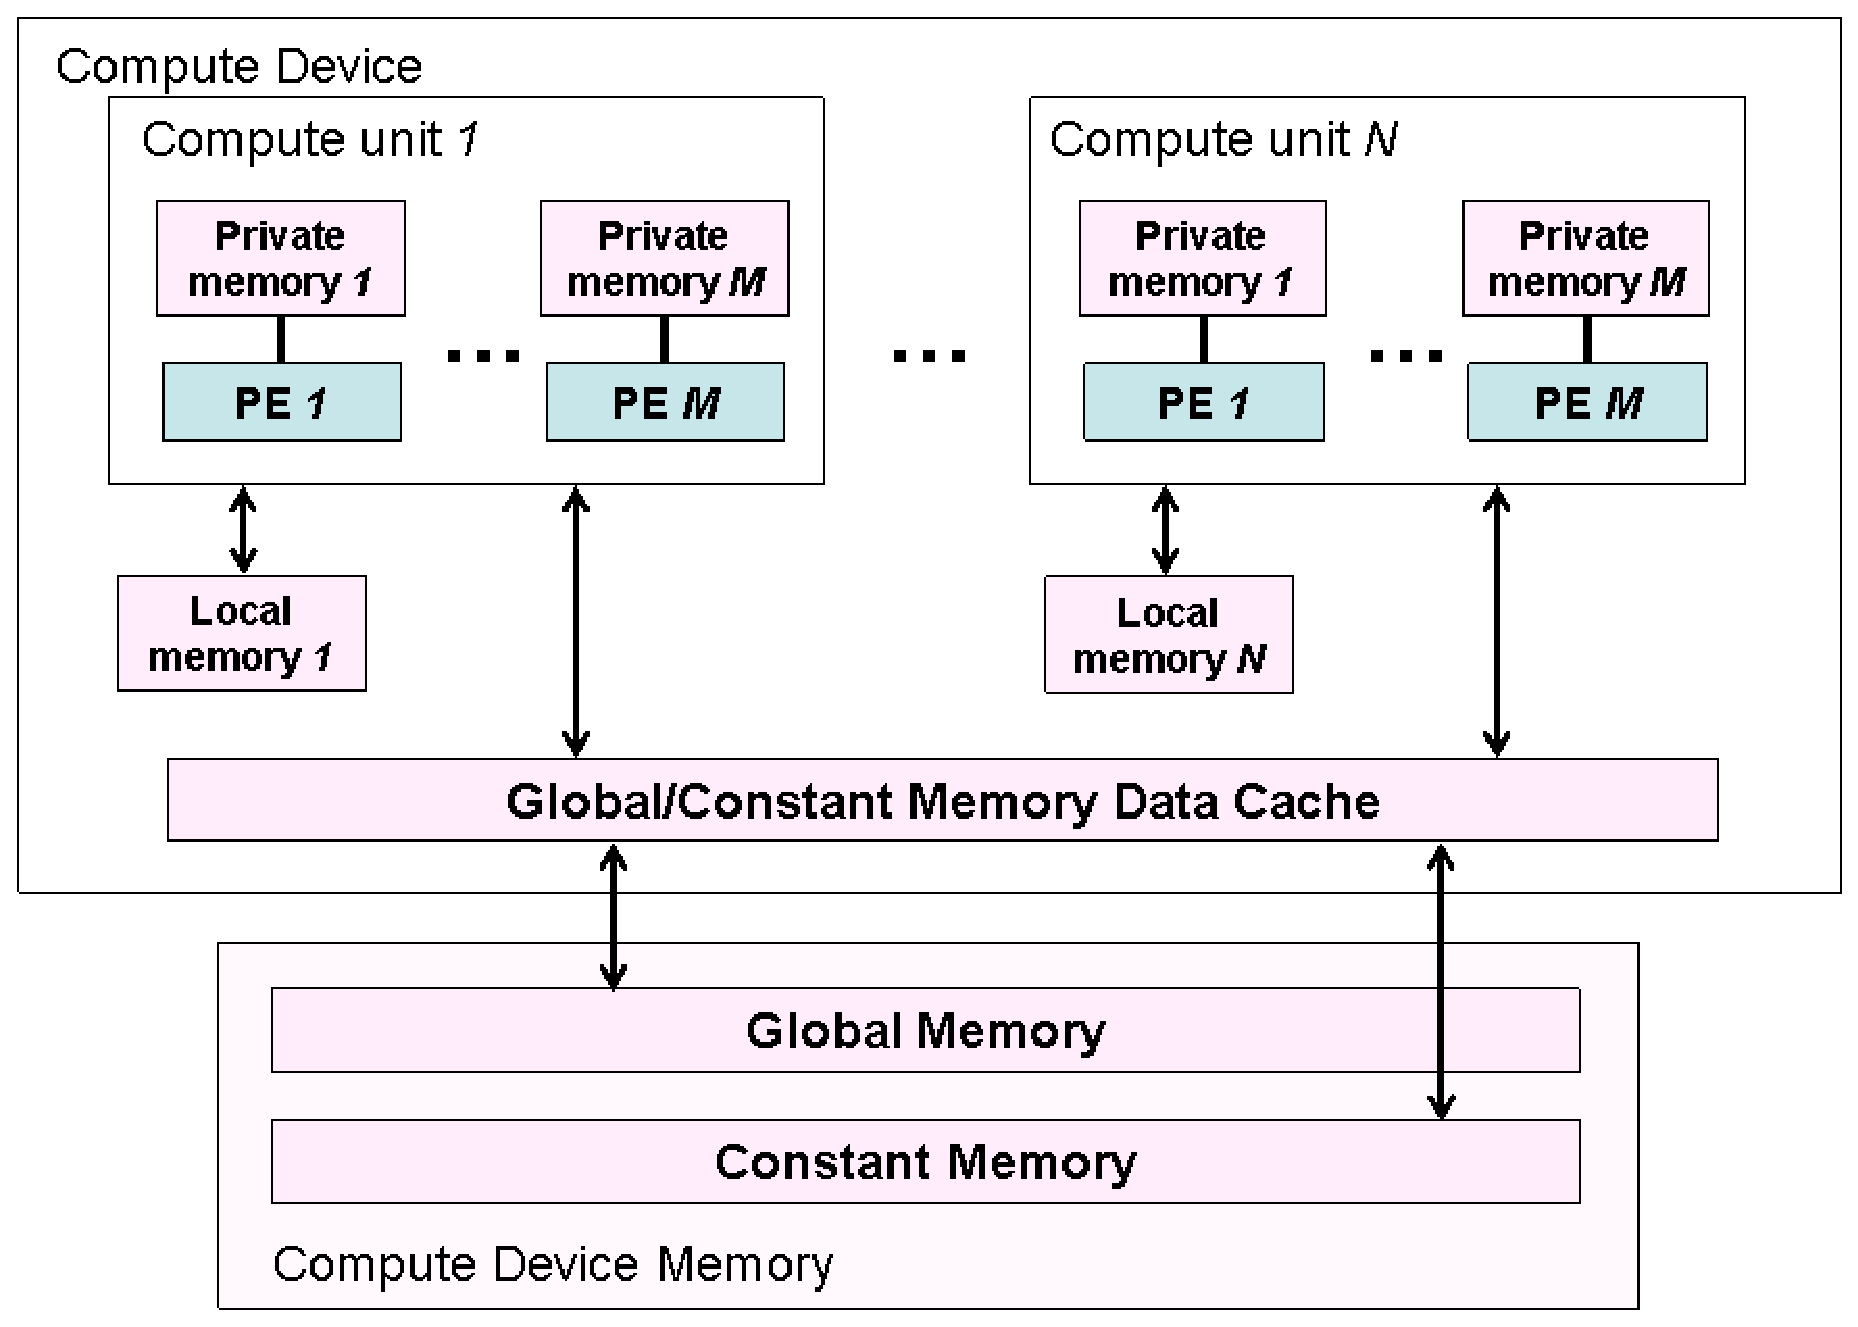
\includegraphics[width=0.6\columnwidth]{figures/eps/device.eps}
		\caption{OpenCL device architektúra (forrás: \cite{opencl})} 
		\label{fig:device} 
	\end{figure}
	
	
\section{OpenCL programozási modell}
	
	A programozási modell a hozzá tartozó osztálydiagrammon (\ref{fig:class}. ábra) figyelhető meg.
	
	\begin{figure}[!ht]
		\centering
		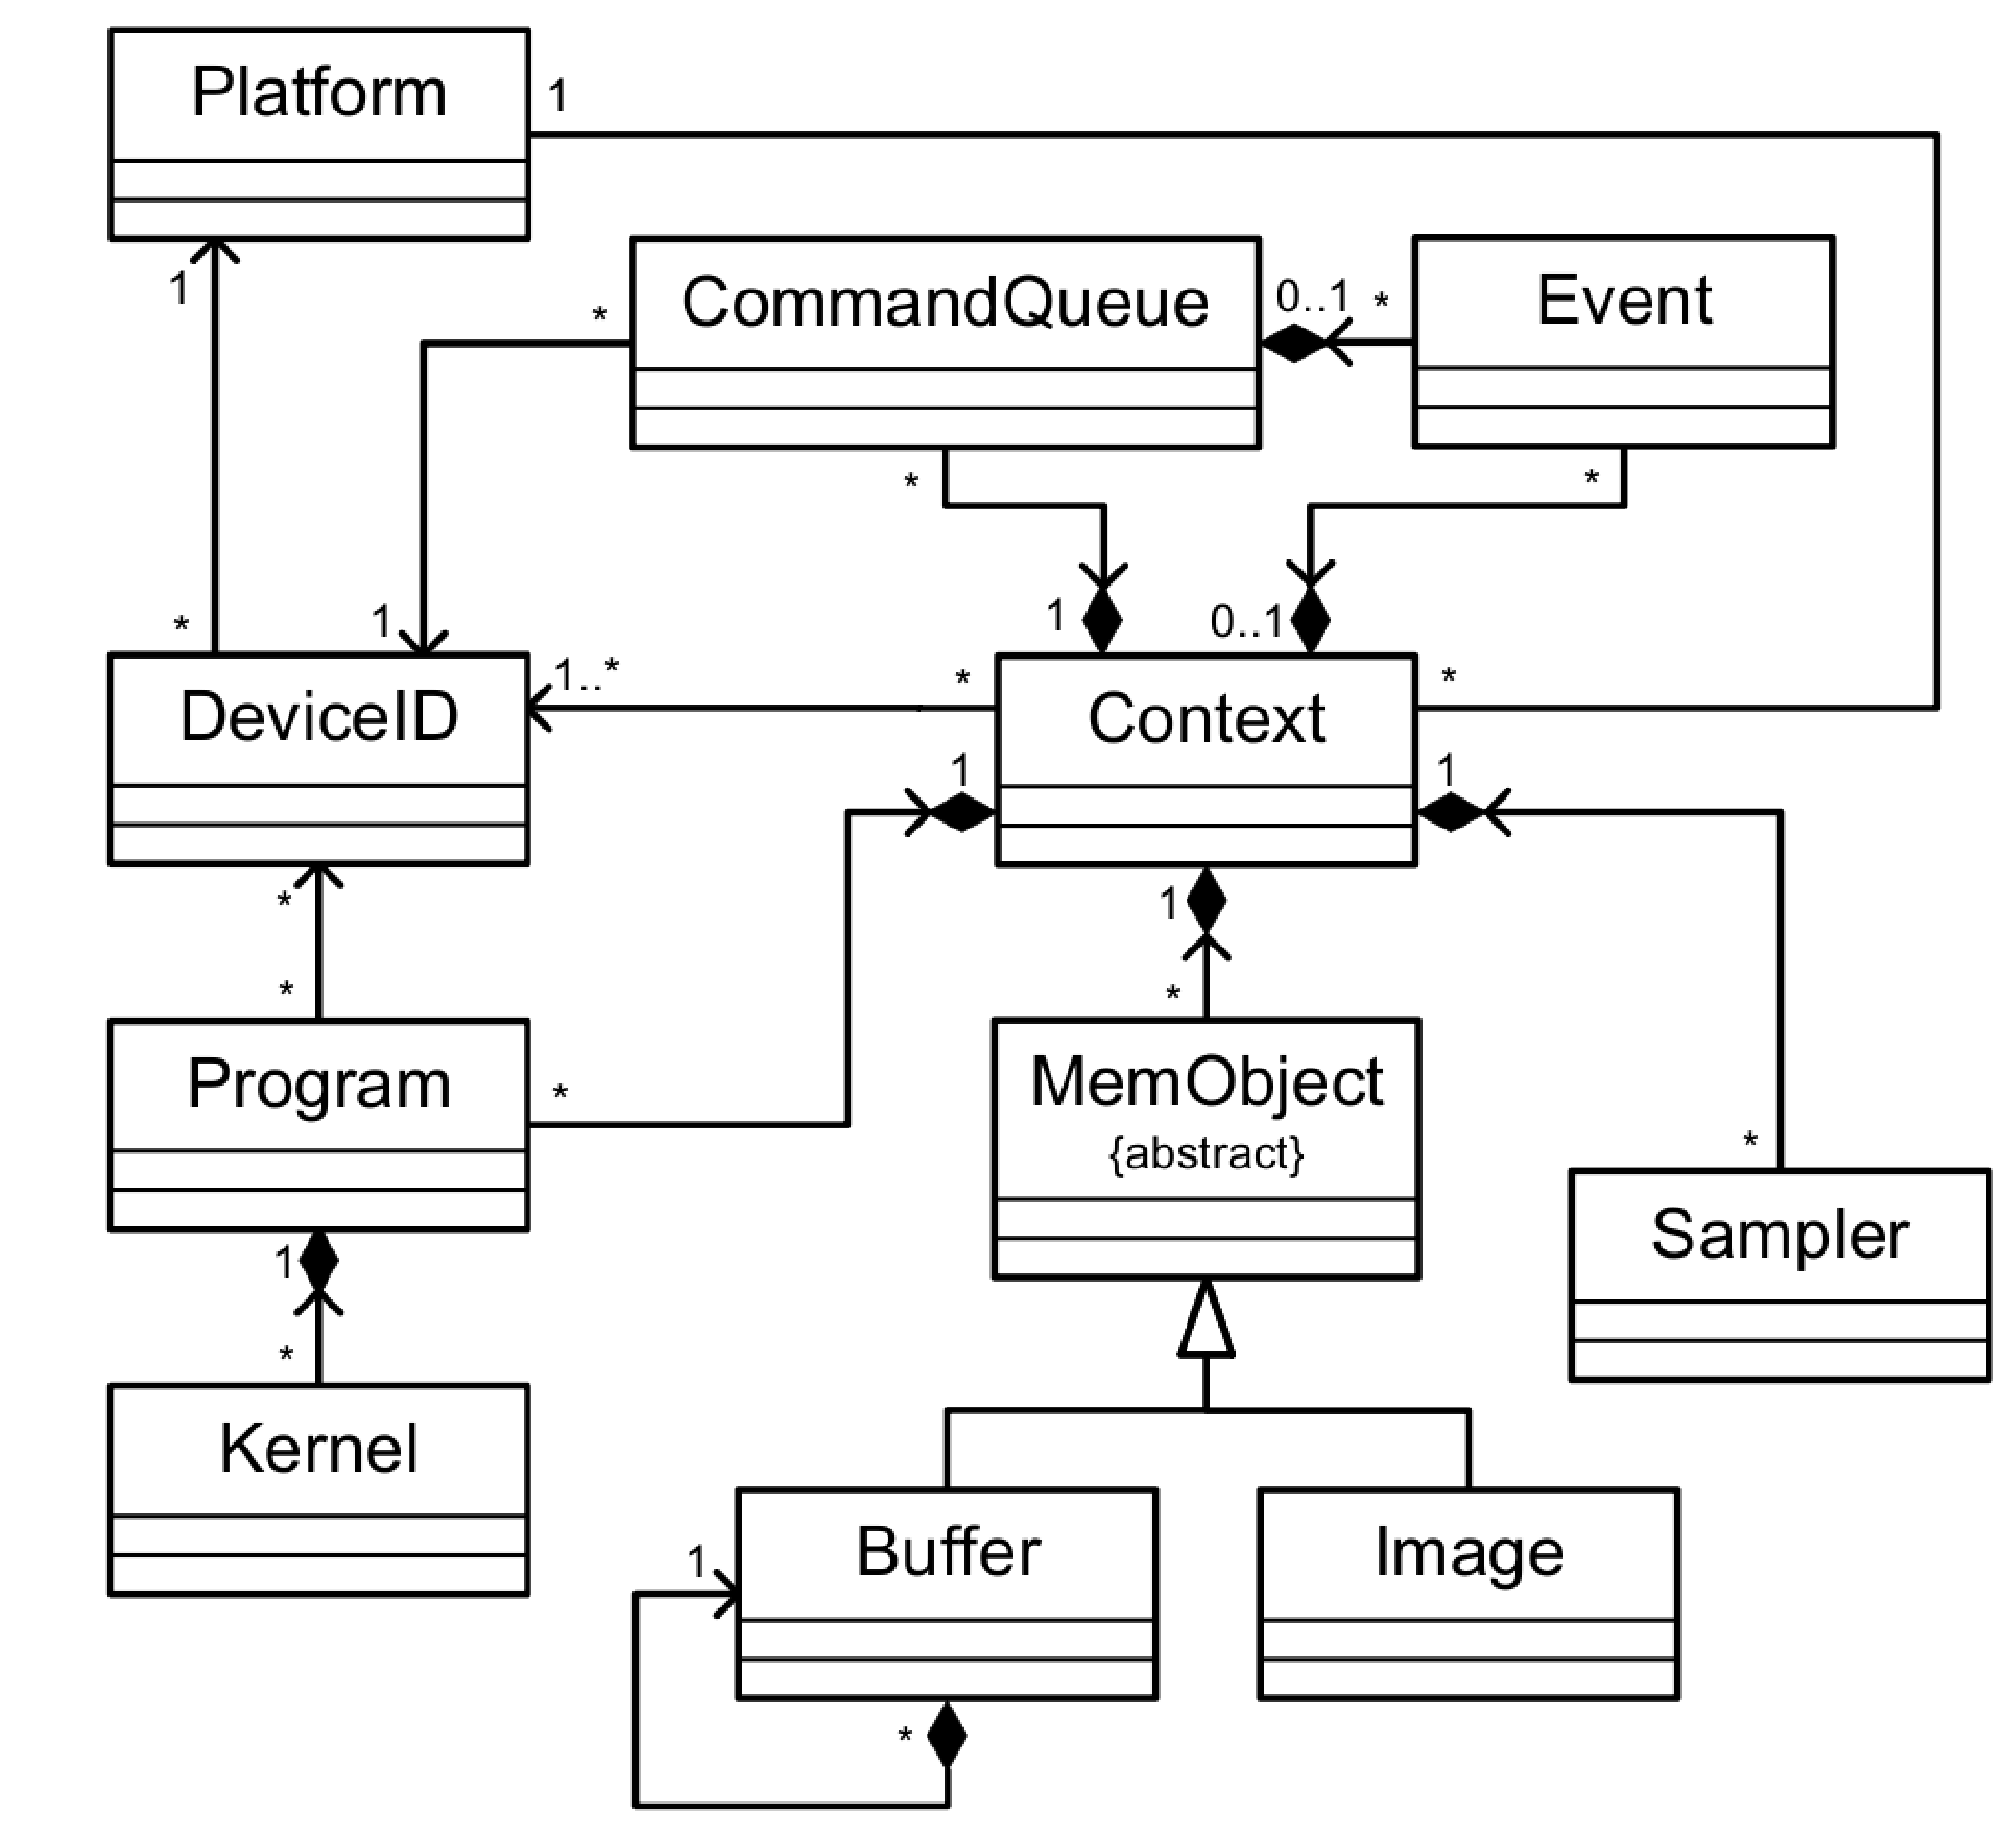
\includegraphics[width=0.6\columnwidth]{figures/eps/context.eps}
		\caption{OpenCL context osztálydiagrammja (forrás: \cite{opencl})} 
		\label{fig:class} 
	\end{figure}
	A futtatáshoz szükséges, hogy a kontextushoz platformot, majd azon belül
	eszközt, az eszközhöz programot (kernelt) és memóriát rendeljünk.
	Figyelembe kell vennünk azt a megkötést, hogy csak az egy platformon belüli
	eszközök programozhatóak heterogén módon. Például: Intel platform esetén
	lehetséges CPU-t, processzorkártyát és Intel-es GPU-t programozni, viszont nVidia kártyákat már nem.
	
	A programozással megoldandó problémát kétféleképpen lehetséges a feldolgozó
	egységekhez (work-item) avagy processzorokhoz rendelni:
	adat parallel módon vagy taszk parallel módon.
	
	Adat parallel módon (\ref{fig:data_parallel} ábra) a feldolgozandó adat egy
	részéhez rendelünk egy feldolgozó egységet. Fontos figyelembe venni az eszköz korlátos
	számú feldolgozó egységének számát. Ha nem elég a feldolgozó egysége akkor a
	feladat megfelelő partícionálásával lehetséges kordában tartani a szükséges
	erőforrás számát.
	
	Taszk parallel módot (\ref{fig:task_parallel} ábra) olyan esetben célszerű
	használna, ha a bemenet dinamikus mérete a futási időben rendkívül változik
	illetve a végrehajtandó feladat lazán függenek össze.
	
	\begin{figure*}[!ht]
		\centering
		\subfloat[Adat parallel]{
			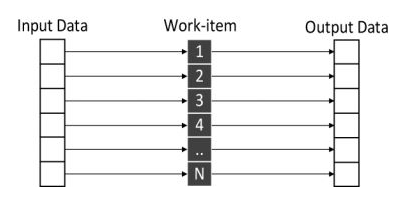
\includegraphics[width=0.45\columnwidth]{figures/eps/data.eps}%
			\label{fig:data_parallel}
		}
		\hfil
		\subfloat[Taszk parallel]{
			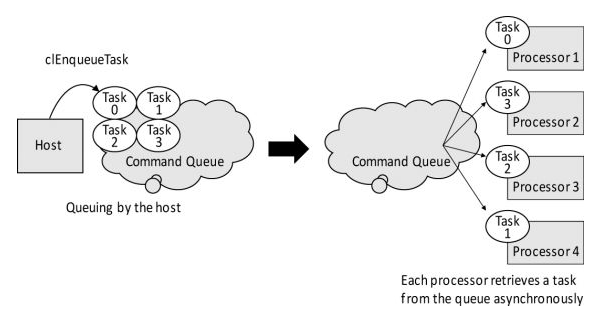
\includegraphics[width=0.45\columnwidth]{figures/eps/task.eps}%
			\label{fig:task_parallel}
		}
		\caption{Feladat hozzárendelése work-item-hez (processzorhoz)}
		\label{fig:parallel}
	\end{figure*}
	A processzor-magok megfelelő kihasználtságának elérése végett több ezer
	work-item virtuálisan osztozik rajta.
	Ezen work-item-eket work-group-okba rendezzük.
	\todo[prepend]{Írni a csoportbarendezés motivációjáró >> SIMD \& vector}
	A work-itemeket jelen pillanatban az OpenCL specifikációja \cite{opencl} szerint $3$ dimenziós
	work-group-ba tudjuk rendezni. Egy példát láthatunk egy work-item indexének a globális és lokális megfelelőjére a
	követekző \ref{fig:ndrange}. ábrán.
	
	\begin{figure}[!h]
		\centering
		\includegraphics[width=0.9\columnwidth]{figures/eps/ndrange.eps}
		\caption{2D-s work-item-ek work-group-ba rendezése és indexelése (forrás: \cite{opencl})} 
		\label{fig:ndrange} 
	\end{figure}
	
	
	Az OpenCL a fizikailag kialíkított memóriákat négy kategórába sorolja a tipikus memóriák kategorizálása a következők:
	\begin{itemize}
		\item \emph{Regiszterek:} Private memory,
		\item \emph{Chipen belüli memória (cache):} Local memory,
		\item \emph{Chipen kívüli memória:} Global memory és Constant Memory.
	\end{itemize}
	A privát és a lokális memória kis méretűnek és gyors elérésűnek mondható, míg a globális és konstans memória nagynak, de
	lassú elérésűnek.
	A definiált memória szintek tipikus paraméterei a következők:
	\begin{itemize}
	 	\item \emph{Privát memória:} minden szálnak külön van, amit a compiler menedzsel.
		\item \emph{Globális és konstans memória:}  Bank szervezés jellemző rá, gyors, de nagy késleltetéssel bír. 8 műveletet
		tud egy ciklus alatt végrehajtan, de csak a parancs kiadása után 400-800 ciklus késleltetéssel. Ha az adaton végrehajtandó
		műveletek ideje ennél jóval nagyobb, akkor ezt a késleltetést el lehet rejteni. 
		\item \emph{Lokális memória:} Minden work-group-nak sajátja van. Minimális a késletetés, sebessége nagy (38-44 GB/s).
		\item \emph{Host memória:} Nagy méretű, közepes sebességű, de sebességét a host-ot és a device-t összekötő PCIe interfész
		korlátozza.
	\end{itemize}
	A memóriákra megkötésként szolgál, hogy ki allokálhat, írhat és olvashat belőle. A \ref{table:mem}. táblázatban látható ezen
	jogosultságokat és a főbb tulajdonságokat.
	
	\begin{table}[!h]
	\renewcommand{\arraystretch}{1.3}
	% if using array.sty, it might be a good idea to tweak the value of
	% \extrarowheight as needed to properly center the text within the cells
	\caption{OpenCL memória szintek}
	\label{table:mem}
	\centering
	% Some packages, such as MDW tools, offer better commands for making tables
	% than the plain LaTeX2e tabular which is used here.
	\begin{tabular}{l|l|l|l|l}
			 & Host memory & Global memory & Local mem. & Private mem.\\ \hline
		Host & Dinamikusan R/W & Din. R/W &  Din. R/W & - \\
		Kernel & - & R/W & Satik. R/W & Statik. R/W\\
		Sebesség & Lassú & Közepes & Gyors & Regiszter\\
		Méret & $4$ Gb $\leq$ & $1$ Gb $\leq$ & $16,32$ Kb & $<1$ Kb
	\end{tabular}
	\end{table}

	A work-group-okba rendezés a lokális memória jogusultsága miatt érdekes.
	Konkrétan az egy work-group-ba tartozó összes work-item azonos lokális memórián
	osztozik.
	Ennek a következménye az, hogy adat parallel módú feldolgozás esetén
	az egymásra ható adatokhoz tartozó work-item-eket egy work groupba kell
	rendelnünk.
	Ha ez nem lehetséges, akkor a globális memóriához kell fordulnunk.
	A globális memória avagy a bank szervezésű külső (off-chip) memóriák
	hozzáférési ideje relatíve nagy így ezek használatát lehetőleg el kell kerülni
	és a programozónak kell ``cachelni" a lokális memóriába.
	
	Mivel a work-item-ek konkurrensen hajtódnak végre, így az általuk közösen elérhető memóriákra
	(globális, lokális) nézve versenyhelyzetben vannak.
	Az OpenCL ezt a problémát a laza memóriamodell használatával oldja meg.
	Work-item-ek közötti szinkronizációra egy korlátot alkalmaz a programban, amit csak akkor léphet át, ha az összes többi
	work-item (az azonos work-group-ban) ezt a korlátot már elérte.
	Erre a \texttt{barrier(FLAG)} függvényhívás szolgál. Fontos megjegyezni, hogy ez a szinkronizáció csak egy adott
	work-group-on belül történik, a work-group-ok közötti és akülönböző work-group-okon belüli work-item-ek szinkronizációra nincs
	lehetőség.
	
	\begin{center}
		Összefoglalva: nagy hangsúlyt kell a memóriaszervezésre fordítani, hogy a processzormagok megfelelően legyenek az adatokkal
		táplálva az elérhető számítási kapacitás kiaknázása végett.
	\end{center}


\section{Futási környezet bemutatása}
	A következő eszközök teljesítményét vizsgálom:
	\begin{itemize}
		\item A laptopomban található \textbf{Intel Core i5 M520} processzor,
		\item A laptopomban található kis teljesítményű \textbf{nVidia GT330M} videókártya,
% 		\item Asztali PC-ben található \textbf{Intel Xeon CPU},
% 		\item Asztali PC-ben található \textbf{Intel Xeon Phi} co-processzor \cite{phi,mic}. 
	\end{itemize}
	Ezen eszközök legjelentősebb paraméterei a \ref{table:envs} táblázat tartalmazza.
	
	\begin{table}[!ht]
	\renewcommand{\arraystretch}{1.3}
	% if using array.sty, it might be a good idea to tweak the value of
	% \extrarowheight  as needed to properly center the text within the cells
	\setlength{\extrarowheight}{8pt}
	\caption{Használandó eszközök összehasonlítása}
	\label{table:envs}
	\centering
	\footnotesize
	% Some packages, such as MDW tools, offer better commands for making tables
	% than the plain LaTeX2e tabular which is used here.
% 	\begin{tabular}{ l | r | r | r | r}
% 		 & Intel Core i5 & nVidia GT330M & Intel Xeon & Xeon PHI \\ \hline
% 		MAX COMPUTE UNITS & $4$ & $6$ & $8$ & $224$\\
% 		MAX CLOCK FREQUENCY & 2400 & 1265 & 3000 & 1100\\
% 		MAX WORK GROUP\_SIZE & $8192$ & $512$ & $8192$ & $8192$ \\ \hline\hline
% 		GLOBAL MEM SIZE & $\sim 4Gbyte$ & $1Gbyte$ & $8Gbyte$ & $\sim 4.5Gbyte$\\
% 		%MAX\_CONSTANT\_BUFFER\_SIZE & $131072$ & $65536$ & $131072$ & $131072$\\
% 		LOCAL MEM SIZE & $32 Kbyte$ & $16 Kbyte$ & $32 Kbyte$ & $32 Kbyte$\\
% 	\end{tabular}
	
	\begin{tabular}{ l | r | r}
		 & Intel Core i5 M520 & nVidia GT330M \\ \hline
		MAX COMPUTE UNITS & $4$ & $6$\\
		MAX CLOCK FREQUENCY & $2400$ MHz & $1265$ MHz \\
		MAX WORK GROUP\_SIZE & $8192$ & $512$ \\ \hline\hline
		GLOBAL MEM SIZE & $4GB\ (2GB)$ & $1GB\ (768 MB)$\\
		%MAX\_CONSTANT\_BUFFER\_SIZE & $131072$ & $65536$ & $131072$ & $131072$\\
		LOCAL MEM SIZE & $32 KB$ & $16 KB$\\
	\end{tabular}
	\end{table}
	
	Az összehasonlíthatóság végett a legkissebb memóriájú eszközre fogom a problémát skálázni, ami a
	GT330M videókártya. A CPU memóriája jóval nagyobb, így a kód mindegyiken tud futni.






% ----------------------------------------------------------------------------
\chapter{Multiprocesszoros program}
% ----------------------------------------------------------------------------
\section{A szimulátor dekomponálása a párhuzamos feladatokra}

\section{A szimulátor bemutatása} 
	 A prototípus algoritmus fejlesztése MATLAB környezetben történt, ami a későbbi referenciaként szolgál.
	 Alap MATLAB utasításokat használva több órát vesz igénybe a szimuláció futtatása.
	 A MATLAB Parallel Toolbox-nak segítségével a szimulációt lehetséges párhuzamosan több processzormagon futtatni.
	 Ezzel párszoros sebesség növekezés érhető el a MATLAB magas nyelvű programnyelve végett.
	 A következőkben magát az algoritmust és az OpenCL keretrendszerben történő implementációját mutatom be.
	 Majd az eredmények bemutatása után összevetésre kerül a MATLAB referencia, a MATLAB Parallel Toolbox segítséggel,
	 az OpenCL processzoron és az OpenCL GPU-n való futási ideje.
	
\section{A lépések részletezése} 
\subsection{Interpoláció}
	A korábban elmondottak alapján a felületet további virtuális pontokkal egészítjük ki.
	Az virtuális mérési pontokat a legegyszerűbben bilineáris interpolációval (síklapos közelítéssel) becsülhetjük.
	\begin{changebar}
	A szimulátorban egy általánosabb módszert alkalmazunk, ami egy 2D-s mozgó átlagoló szűrővel való simítás.
	A szűrővel aluláteresztést tudunk elérni, ami a minta magasságának mintavételezése utáni rekonstrukcióját jelenti.
	\end{changebar}
	Egy ilyen interpoláció eredményét láthatjuk a \ref{fig:33pont}. ábrán.
	
	\begin{figure}[!h]
		\centering
		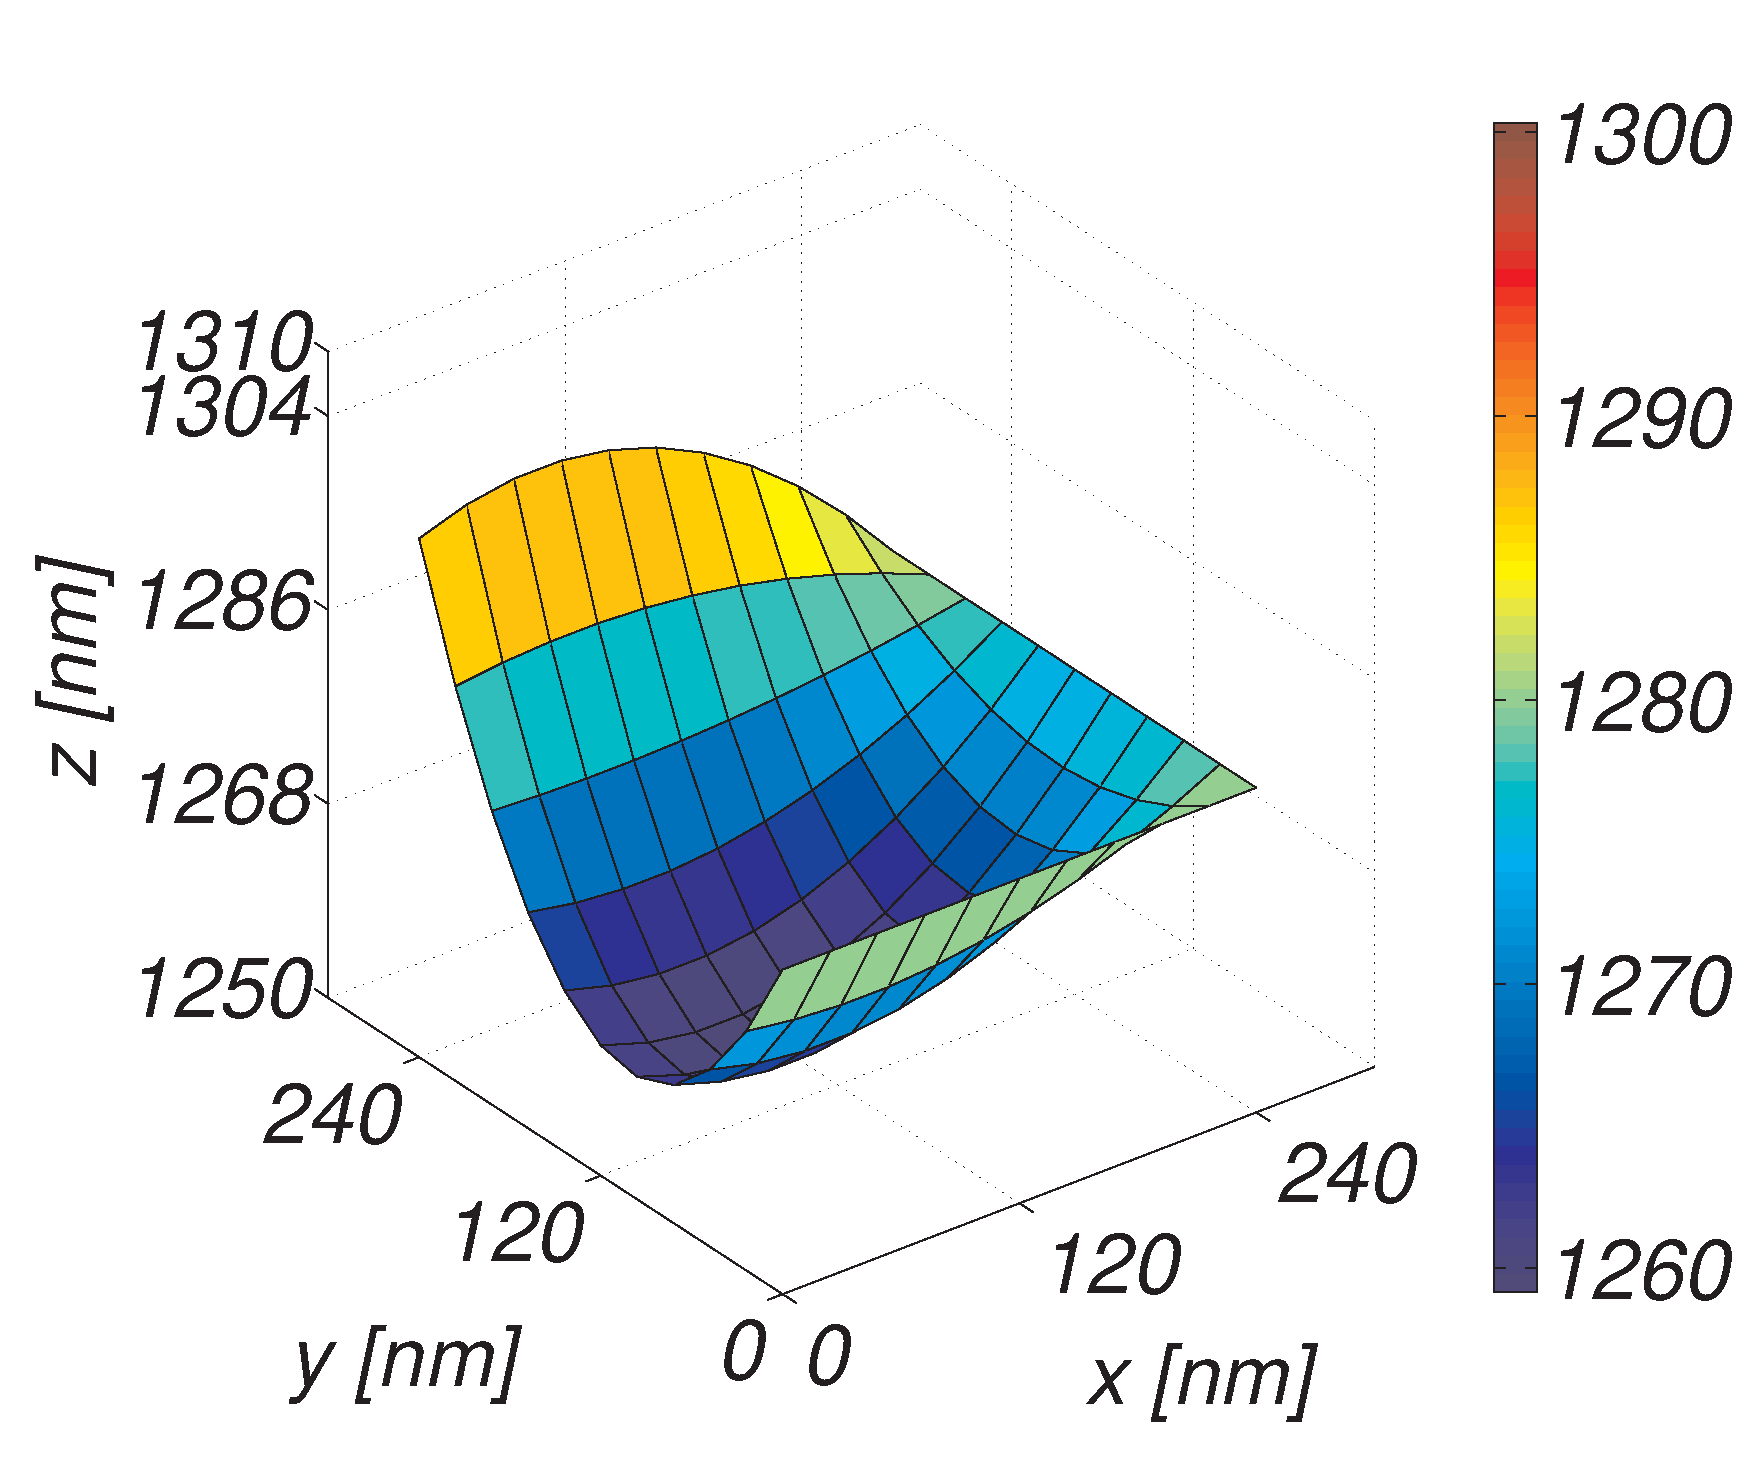
\includegraphics[width=0.8\columnwidth]{figures/eps/3x3_interpol2.eps}
		\caption{$3\times3$ mérési pont $11\times11$ pontba való interpolációja}
		\label{fig:33pont}
	\end{figure}
	
\subsection{Szimulálandó térfogat méretének számítása}
	A szimulálandó tér (hasáb) alapja adott az előzőleg említett interpolált felületként, míg a
	magassága nem. Ezt a következő két mennyiség közül a nagyobbikkal határoztuk meg:
	\begin{itemize}
		\item Középső pont fölött lévő tű közepének magassága,
		\item A ($3\times3$) környezet legalacsonyabb és legmagasabb pontjának
		különbsége.
	\end{itemize}
	A magasságtérkép egy vonalának részlete látható a \ref{fig:numh}. ábrán, 
	továbbá a szimulálandó tér (hasáb) magassága.
	
	\begin{figure}[!ht]
		\centering
		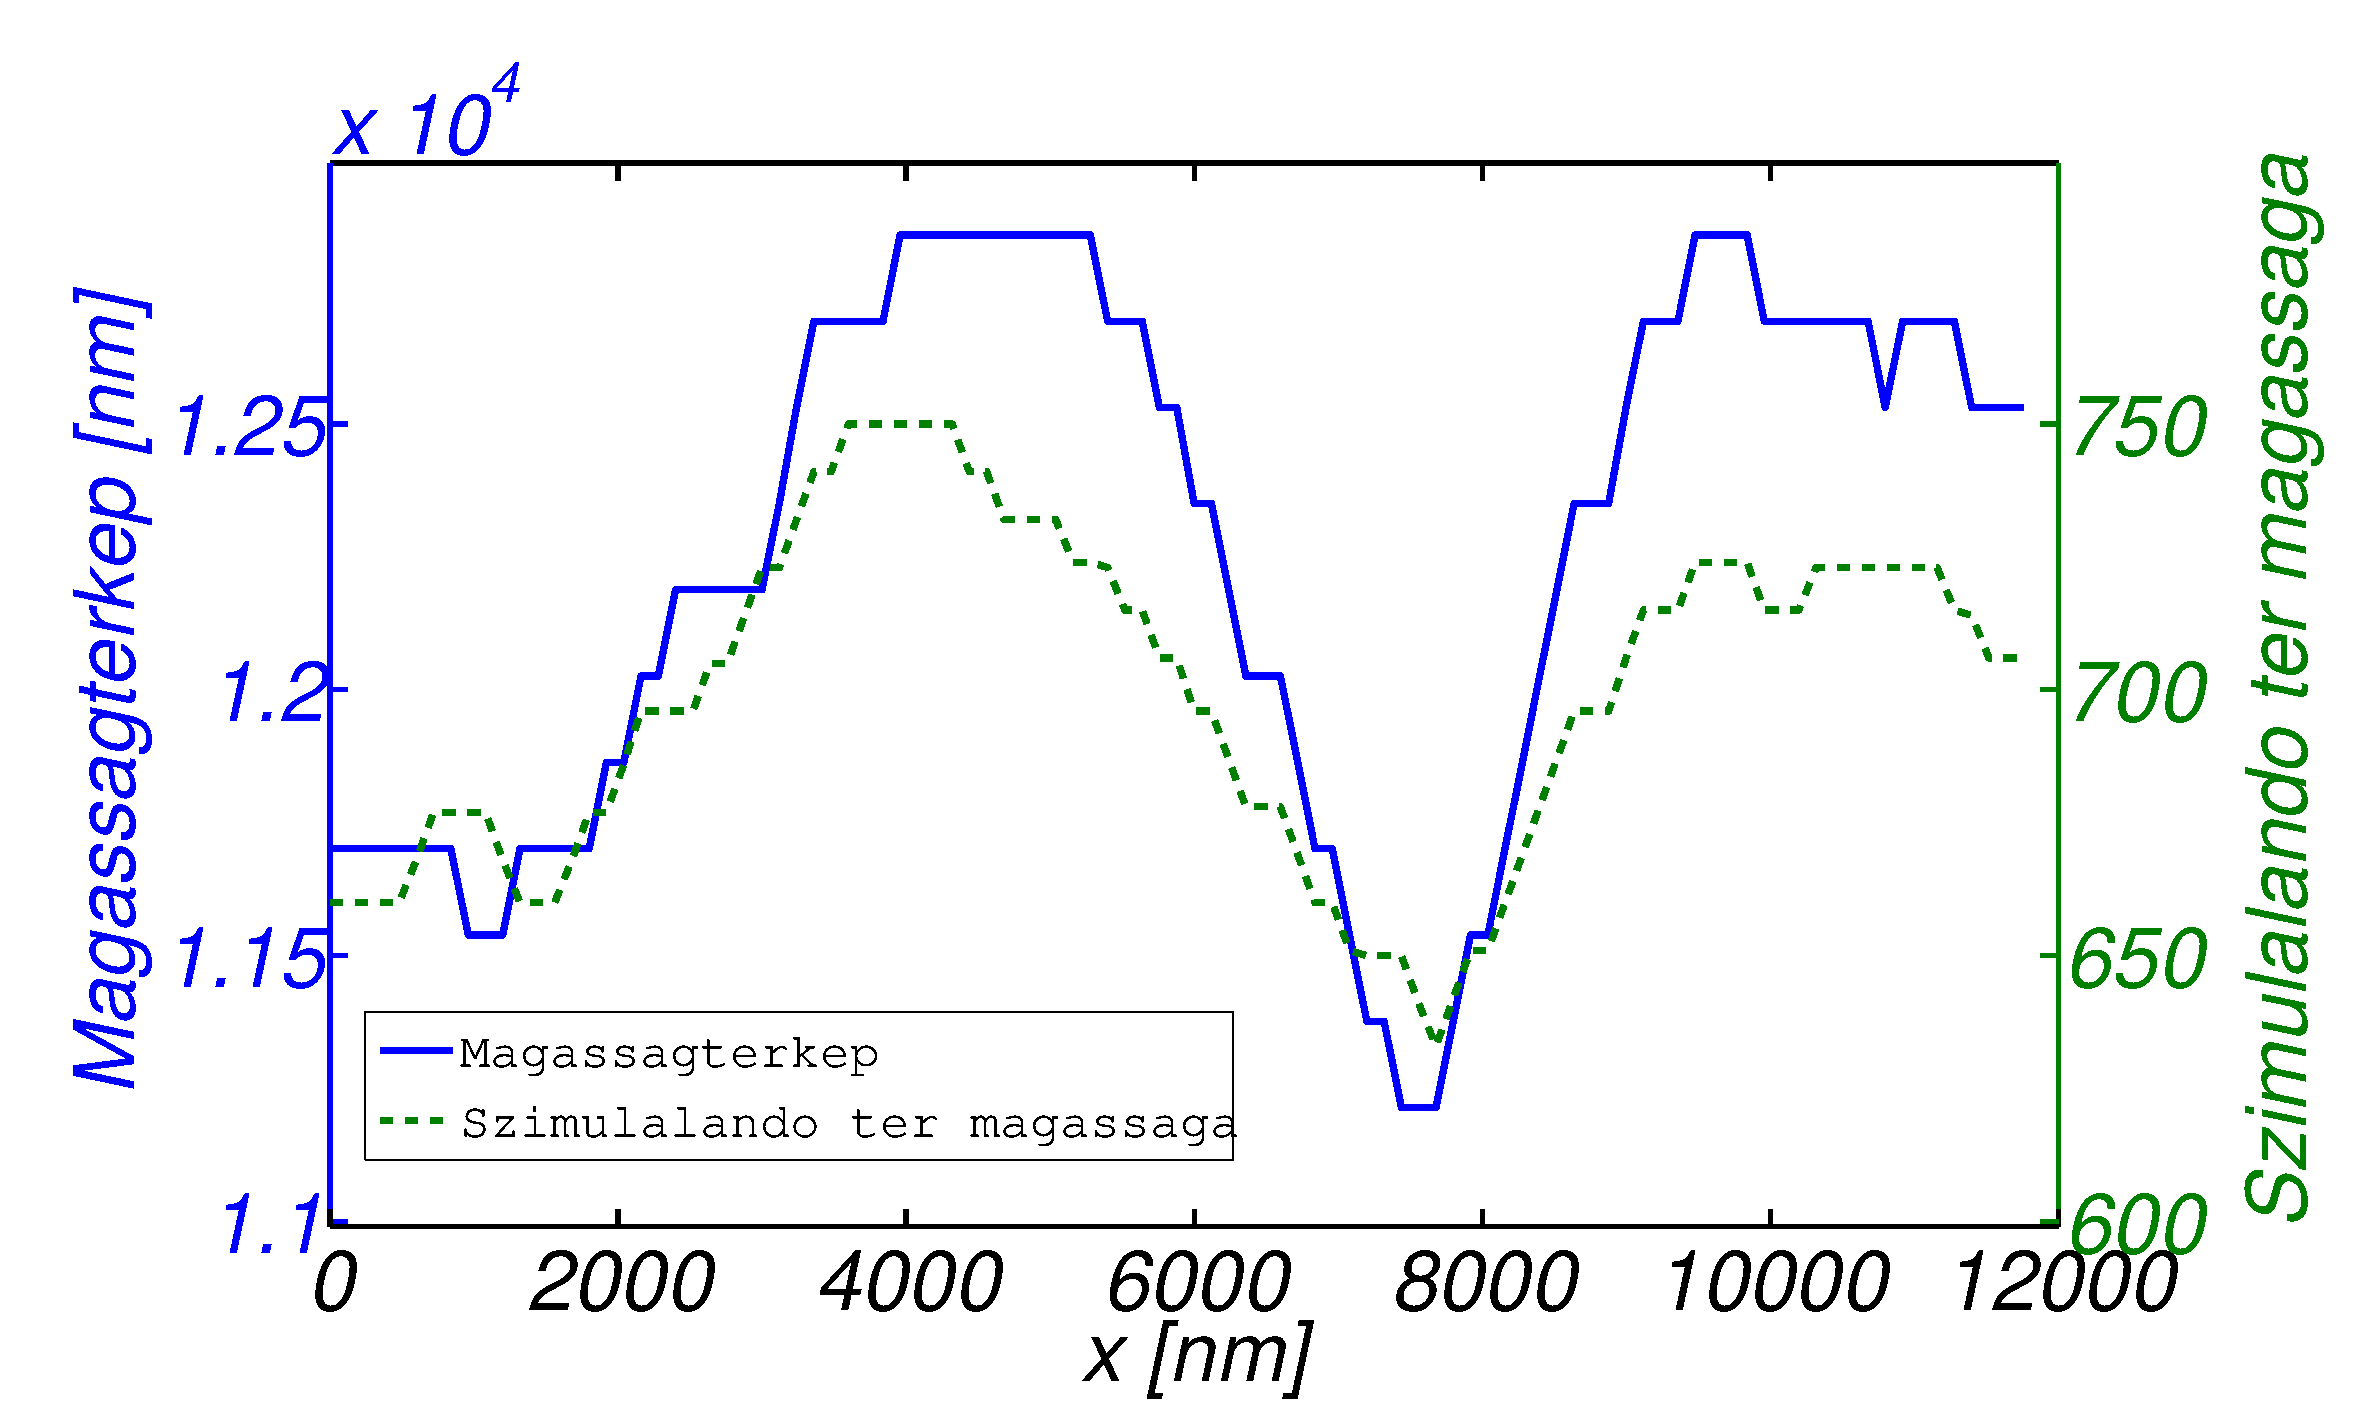
\includegraphics[width=0.7\columnwidth]{figures/eps/numh_vonal.eps}%
		\caption{A mérési eredmény egy vonal menti részlete (folytonos vonal) és az ezen
		mérési pontokhoz számított szimulációs tér magassága (szaggatott-vonal)}
		\label{fig:numh} 
	\end{figure}

	
\subsection{Iteratív megoldó algoritmus}
	Az iterációhoz a térháló pontjaihoz két mátrixot (tömbböt) rendelünk, ami a
	pontok potenciáljának aktuális ($\mathbf{V_{now}}$) és előző ($\mathbf{V_{prev}}$)
	értékeit tartalmazza.
	Az aktuális értékeket \eqref{eq:it} szerint számítjuk, majd az egész térre
	számítjuk az előzővel vett különbségének négyzetösszegét (normáját). E mérték
	képviseli a konvergencia szintjét, amit az iteráció során vizsgálva jutunk el a
	kívánt konvergencia szintre.
	Ha nem értük el a konvergencia szintet, akkor az előző két mátrixot
	felcserélve iterálunk tovább.
	
\subsection{Adatok mentése}
	Tesztelhetőségi megfontolások végett nem csak a tűre ható erőt (villamos
	térerősséget) exportáljuk, hanem a konvergencia szintjének változását és az
	interpolált felületet is. Az exportálandó menyiségek ``kis''
	mérete miatt egyszerű *.csv fájlként kerülnek mentésre. Ezen fájlok további
	poszt-processzálása MATLAB vagy munkalap kezelő szoftverrel is elvégezhető.

\section{Implementációhoz szükséges megfontolások}
	
	A következőkben egy kissebb teljesítményű notebook videókártyát veszek
	alapul a megfontolások demonstrálására. Ez az nVidia GeForce 330M, 
	575 MHz-en futó 48 CUDA core-al, 1024GB memóriával és
	OpenCL 1.0 kompatibilitással.
	A videókártya továbbiakban fontos paraméterei a \ref{table:vcard}. táblázatban
	látható.
	
	\begin{table}[!h]
	\renewcommand{\arraystretch}{1.3}
	% if using array.sty, it might be a good idea to tweak the value of
	% \extrarowheight as needed to properly center the text within the cells
	\caption{nVidia GeForce 330M OpenCL tulajdonságai}
	\label{table:vcard}
	\centering
	% Some packages, such as MDW tools, offer better commands for making tables
	% than the plain LaTeX2e tabular which is used here.
	\begin{tabular}{l|r}
		MAX\_COMPUTE\_UNITS & 6\\
		MAX\_WORK\_GROUP\_SIZES & 512 512 64\\
		GLOBAL\_MEM\_SIZE & 1073020928\\
		MAX\_CONSTANT\_BUFFER\_SIZE & 65536\\
		LOCAL\_MEM\_SIZE & 16384
	\end{tabular}
	\end{table}
	
	Ha a tér, ahol a laplace egyenletet meg kell oldanunk nagyon nagy, akkor
	érdemes szétbontani kissebb alterekre és azokhoz rendelni egy-egy
	``work-item''-et. Mivel a diszkrét Laplace egyenlet egy pontja a szomszédos
	pontokkal szoros kapcsolatban van, így az összefüggő ``work-item"-eket egy
	``work-group''-ba érdemes szervezni, mivel így az átlapolódó pontok értékét a
	szomszédos ``work-item''-ek is tudják írni és olvasni. Az ilyen típusú
	problémának méretét a MAX\_WORK\_GROUP\_SIZES tulajdonság korlátozza.
	
	Jelen esetben a mérési eredmény egy pontjához tartozó tér átlagosan
	$11\times11\times30$ pontból áll.
	Tehát a korábbi nem áll fenn és egyszerű megfeleltetéssel szétoszthatjuk a
	feladatot.
	A teljes tér $512\times512\times11\times11\times30$ méretű, ami $951k$ pont.
	A tárolásához single-precision mellett ennek a számnak a 4-szerese
	szükségeltetik byte-okban mérve. Mivel ez a videókártyán nem áll
	rendelkezésre, így szétbontjuk kissebb feladatrészekre.
	
	Ezen feladatrészek méretét egy paraméter állításával lehet változtati és az
	implementált algoritmus ettől generikusan függ.
	Emellett az interpoláció mértéke $N_{ip}$ is paraméterrel generikusan állítható.
	Az algoritmus generikusságát csupán a futási időben történő dinamikus memória
	allokációval lehetséges megvalósítani. A korábban említettek végett (\ref{table:mem} táblázat)
	az allokáció csak a ``host'' programban történhet.

\section{Memória szervezés}
\subsection{Csak globális memória használata}
	Az algoritmus pszeudó kódjának direkt leképezése esetén a ``host''-on
	allokálunk memóriát a ``device'' globális memóriájában,
	majd a megfelelő adatokat ide másoljuk és a kernel is itt ír és olvas.
	A problémát a globális memória nagy hozzáférési ideje jelenti, ami miatt sok
	``work-item'' tétlenül a memóriára fog várakozni.
	Ilyenkor az egy mérési pontra vonatkoztatott szimulációs idő a
	referenciánál is lassabb.
\subsection{Globális memória és adott esetben lokális memória használata}
	Kis erőfeszítéssel nagy javulást lehet elérni, ha a mérési ponthoz tartozó
	szimulációs tér éppen belefér a lokális memóriába.
	Tehát, mielőtt az \eqref{eq:it} szerinti iteratív megoldót futtatnánk először a
	globális memóriából a lokális memóriába töltjük át a kérdéses pontokat, majd
	számolunk rajta és a végén visszatöltjük a globális memóriába.
	E javítással a referenciával azonos sebességet tudunk elérni.
\subsection{Globális memória és minden adódó alkalomkor a lokális memória használata}
	Nagyobb erőfeszítést igényel, hogy minden alkalommal a globális memóriával való kommunikációt a
	lokális memória közbeékelésével tegyük.
	Ezt úgy lehet felfogni, mintha a globális memóriát lokális memória méretű
	kvantumokban tudnám csak elérni.
	Ekkor nagy odafigyelést kíván a memóriacímzés megfelelő prgramozása, de
	eredményképp gyorsulás érhető el. \\
	
	\noindent
	\begin{center}
	Összegezve elmondható, hogy az aktuálisan használt adat tárolását a lehető
	legközelebb kell tartani a ``compute-unit''-hoz.
	\end{center}
	
	\begin{table*}[!Ht]
		%\renewcommand{\arraystretch}{1.2}
		% if using array.sty, it might be a good idea to tweak the value of
		% \extrarowheight as needed to properly center the text within the cells
		\caption{OpenCL futási idő eredmények $12\times12$ mérési pontra}
		\label{table:openresult}
		% Some packages, such as MDW tools, offer better commands for making tables
		% than the plain LaTeX2e tabular which is used here.
		\centering
		\begin{tabular}{l|r|r|r}
		 & Globális memória & Lokális memória, ha befér & Lokális memória bufferelés\\ \hline
		\parbox{2.5cm}{Globális tranzakciók száma átlagosan} & $12 \times 12\times 32.3$
		& $12 \times 12 \times 32.3$ & $12 \times 12 \times 32.3$\\
		\parbox{2.5cm}{Lokális tranzakciók száma átlagosan} & 0 &
		$0.48 \times 12 \times 12 \times 30$ & $2.08 \times 12 \times12 \times 32.3$\\
		Futási idő & 5990 ms & 2530 ms & 510 ms\\
		Fajlagos futási idő & 410 ms & 170 ms & 3.5 ms 
		\end{tabular}
	\end{table*}
	
%----------------------------------------------------------------------------
\chapter{Konvergencia vizsgálata}
%----------------------------------------------------------------------------
\section{Interpolációk közötti különbségek}




\section{Különböző alap formák esetén}





%----------------------------------------------------------------------------
\chapter{Eredmények}
%----------------------------------------------------------------------------
	\section{MATLAB implementációk}
	A referenciaként szolgáló MATLAB algoritmus lineáris programszervezést
	alkalmazva az elérhető fajlagos futási idő $\sim100 ms$.
	
	A kód minimális változtatásával elérhető a párhuzamos végrehajtás. Ezt a
	\texttt{for} ciklusok Parallel Toolbox beli \texttt{parfor} utasítására
	cserélve érhetjük el. 4 processzormaggal rendelkező PC-n  legjobb esetben a negyedére csökkenhet a
	futási idő. Valójában ez sose történik meg.
	A MATLAB Parallel Toolbox-a az egyes szimulácókat adott processzormagra osztja el.
	Korábban láttuk, hogy ezen szimulációk lépésigénye nagyban eltér egymástól, így előáll az a
	sajnálatos eset, hogy 3 mag tétlenül a negyedikre vár, ami miatt ez nem tekinthető járható útnak. 
	
	\section{OpenCL implementációk}
	OpenCL keretrendszer segítségével írt programot a GPU-n futtatva az
	\ref{table:openresult}. táblázatban látható eredményeket kapjuk.
	Csupán a globális memóriát használva a referenciához képest romlik a
	teljesítmény. Ezt a videókártya prediktív cache nélküli kialakításának és a
	globális memórájának a kiéheztetésének tudhatjuk be.
	A lokális memória használata a futási időt drasztikusan le tudja
	csökkenteni, ami a korábban ismertetett memória szervezési megfontolások
	helyességét igazolja.



xx





	A programot a különböző eszközökön futtatva a \ref{table:results}. táblázatban látható futási
	eredményeket produkálta. A táblázatban látható futási idők 100 futási idő átlaga.
	A táblázathoz felvettem egy fiktív mérőszámot (teljesítmény tényező) a különböző architektúra
	összehasonlítására.
	A mérőszám értéke minél kissebb, annál gyorsabban hajtódik végre egy utasítás.
	\begin{table}[H]
	\footnotesize
	\centering
	\caption[Eszközök futási idejének összehasonlítása]{Az eszközök erőforrásainak és a rajta futtatott
	programok futási idejének összehasonlítása.}
	\label{table:results}
	\setlength{\extrarowheight}{8pt}
% 		\begin{tabular}{ l | r | r | r | r}
% 		 & Intel Core i5 & nVidia GT330M & Intel Xeon & Xeon PHI \\ \hline
% 		MAX COMPUTE UNITS & $4$ & $6$ & $8$ & $224$\\
% 		MAX CLOCK FREQUENCY & 2400 & 1265 & 3000 & 1100\\
% 		MAX WORK GROUP\_SIZE & $8192$ & $512$ & $8192$ & $8192$ \\ \hline\hline
% 		GLOBAL MEM SIZE & $\sim 4Gbyte$ & $1Gbyte$ & $8Gbyte$ & $\sim 4.5Gbyte$\\
% 		LOCAL MEM SIZE & $32 Kbyte$ & $16 Kbyte$ & $32 Kbyte$ & $32 Kbyte$\\ \hline\hline
% 		Futási idő &
% 		\end{tabular}
	\begin{tabular}{ l | r | r}
		 & Intel Core i5 M520 & nVidia GT330M \\ \hline
		MAX COMPUTE UNITS $[1]$ & $4$ & $6$\\
		MAX CLOCK FREQUENCY $[\mathrm{MHz}]$ & 2400 & 1265 \\
		MAX WORK GROUP\_SIZE & $8192$ & $512$ \\ \hline\hline
		GLOBAL MEM SIZE & $\sim 4\ \mathrm{GByte}$ & $\sim 1\ \mathrm{GByte}$\\
		%MAX\_CONSTANT\_BUFFER\_SIZE & $131072$ & $65536$ & $131072$ & $131072$\\
		LOCAL MEM SIZE & $32\ \mathrm{KByte}$ & $16\ \mathrm{KByte}$\\ \hline\hline
% 		Kép mérete & $1024\times 1024$ & $1024\times 1024$ \\ 
		Futási idő $(T)$ & $478.71\ ms$ & $191.94\ ms$\\
		Teljesítmény tényező $\left(P=\frac{1}{\mathrm{UNITS}\times \mathrm{FREQUENCY}}\right)$ &
		$104.16\cdot 10^{-6}$ & $131.75\cdot 10^{-6}$\\
		Fajlagos utasításszám $(T/P)$ &  $4.59\cdot 10^3$ & $1.45\cdot 10^3$ 
	\end{tabular}
	\end{table}
	\noindent Látható, hogy a GPU-n való futtatás közel $666\times$ gyorsulást jelent.
	Ezt két dolognak tudom be:
	\begin{itemize}
		\item \emph{Memória:} A CPU memóriája DDR3 @ 1066 MHz 64 bites busz szélességgel, míg a GPU
		memóriája GDDR3 @ 1066 MHz 128 bites busz szélességgel,
		\item \emph{Processzor mag:} A CPU 4 compute unit-al rendelkezik, ami 4 szálra, ami 2
		processzormagra az Intel HyperThread technológiájával képeződik le, míg a GPU 6 compute unit-al
		rendelkezik, ami 48 CUDA core-ra képeződik le.
	\end{itemize}
	Továbbá figyelembe kell venni, hogy a program futása a többi programmal konkurrensen történik, CPU
	esetén az operációs rendszerrel, GPU esetén a megjelenítéssel.
	



%----------------------------------------------------------------------------
\chapter{Összegzés}
%----------------------------------------------------------------------------
	A cikkben összefoglaltam az AFM felületi töltéssűrűség méréstechnikáját, amiben azonosítottam a
	kapacitás értékének kritikus voltát. Ezidáig a kapacitás értékének a \cite{Hudlet1998,Butt20051}
	szerinti közelítéseket tartalmazó analitikus eredményt lehetett felhasználni.
	
	Feladatként ezen kapacitás értékét számító szimulátor építését tűztem ki, aminek elfogaható időn
	belül kell eredményt szolgáltatnia. A párhuzamosítás lehetősége triviálisan adódott.
	A hordozhatóság és a gyorsabb végrehajtás végett a szimulátort OpenCL 
	környezetben implementáltam, ami a szimulátor heterogén multiproszesszoros környezetben való
	futtatását lehetővé teszi.
	
	Az eredményeket ismertetve a szimulátor futási idejében látványos gyorsulást tapasztaltam, ami
	az érdesebb felületek esetén is elfogadhatóan pontos eredményt tud szolgáltatni. 

	Végül az elkészült programot CPU-n és GPU-n is futtatva a futási idejüket összevetettem és
	azonosítottam a gyorsulás forrását kitérve a processzormagra és a memóriájára.
	
	\section*{További feladatok:}
	\begin{itemize}
		\item A szimuláció felhasználásával történő töltéssűrűség származtatása még várat magára, ugyanígy ezen származtatás
		validálására való mérési összeállítás kidolgolgozása.
		\item A szimulátor magját képező lineáris egyenletrendszer iterációs megoldó konvergenciájának bizonyítása és az alternatív
		direkt megoldó vizsgálata is további feladat.
	\end{itemize}
	
	
	
	


\pagenumbering{Roman}
\setcounter{page}{1}
% \include{acknowledgement}

\chapter{Függelék}


%----------------------------------------------------------------------------
\section{Referencia program}
%----------------------------------------------------------------------------
\texttt{refcode.c}
\begin{lstlisting}[frame=single,float=!ht,caption=A referencia programkódja,label=listing:refprog]
main() { return; }
\end{lstlisting}

 

\listoffigures\addcontentsline{toc}{chapter}{Ábrák jegyzéke}
\listoftables\addcontentsline{toc}{chapter}{Táblázatok jegyzéke}

\bibliography{bib/bakro-tdk-2014.bib}
\addcontentsline{toc}{chapter}{Irodalomjegyzék}
\bibliographystyle{ieeetr}



\label{page:last}
\end{document}
